\documentclass[12pt]{article}
\usepackage[left=1.5cm,right=1.5cm, top = 2cm, bottom = 2cm]{geometry}
\usepackage{graphicx}
\usepackage{natbib}
\usepackage{hyperref}
\usepackage{todonotes}
\usepackage{booktabs}
\usepackage{amssymb}
\usepackage{amsmath}

\newcommand{\sd}{s}
\newcommand{\mean}{\bar{y}}

\usepackage{xr}
\externaldocument{Draft_MEM}

\usepackage{caption}
\captionsetup[table]{name={{\footnotesize Table}}}
\usepackage{caption}
\captionsetup{font=footnotesize}

\begin{document}


\appendix


\renewcommand{\thepage}{S\arabic{page}}
\renewcommand{\thesection}{S\arabic{section}}
\renewcommand{\thetable}{S\arabic{table}}
\renewcommand{\thefigure}{S\arabic{figure}}
% reset counters
\setcounter{page}{1}
\setcounter{section}{0}
\setcounter{table}{0}
\setcounter{figure}{0}

\begin{center}
{\LARGE Supplementary Material: \textit{A statistical assessment of influenza intensity thresholds from the moving epidemic and WHO methods}}

\medskip

{\large Johannes Bracher and Jonas M. Littek}
\end{center}

\renewcommand{\thepage}{S\arabic{page}}
\renewcommand{\thesection}{\Alph{section}}
\renewcommand{\thetable}{S\arabic{table}}
\renewcommand\thefigure{S\arabic{figure}}
\renewcommand\theequation{S\arabic{equation}}

\setcounter{figure}{0}
\setcounter{table}{0}
\setcounter{equation}{0}

\newpage

\section{List of recent use cases}


\begin{table}[h!]
\caption{\footnotesize Published applications of the MEM and WHO methods to estimate intensity thresholds; $m$ is the number of historical seasons used, while $n$ is the number of observations used per season (in the bottom table we always have $n = 1$). The window width for smoothing with a moving average is denoted by $l$ (in the top table we always have $l = 1$). ``Percentiles'' indicates which percentiles were used for the medium, high and very high thresholds, with ``?'' indicating no information was found. Abbreviations: ARI/SARI = (severe) acute respiratory infection; ILI = influenza-like illness; RSV = respiratory syncytial virus.}
\label{tab:literature}
\center
% \vspace{-3mm}
\scriptsize
\begin{tabular}{l l l l l l l}
\toprule
\multicolumn{7}{c}{(a) Moving epidemic method}\\
\toprule
Region & Disease / condition & Years & $m$ & $n$ & Percentiles & Authors\\
\midrule
Africa (25 countries) & influenza & varies & varies & varies & 40, 90, 97.5 & \cite{Igboh2021} \\
Australia & ILI/influenza & 2012--2017 & 5 & 6 & 40, 90, 99 & \cite{Vette2018}\\
Australia, Chile, & ILI/SARI & 2013--2019 & 6 & 5 & 40, 90, 97.5 & \cite{Sullivan2019}\\
New Zealand,\\
South Africa\\
Bangladesh & influenza & 2016--2019 & 4 & 8 & 40, 90, 97.5 & Aba Oud et al (\citeyear{AbaOud2021})\\
Catalonia & ILI & 2010--2016 & 5 & 6 & ? & \cite{Basile2018}\\
Catalonia & ILI & 2005--2018 & 12 & 3 & ? & \cite{Basile2019}\\
Catalonia & ILI/influenza & 2010--2017 & 7 & 4 & ? & \cite{Torner2019}\\
Egypt & SARI/ILI & 2010--2017 & 6 & 5 & 40, 90, 97.5 & \cite{AbdElGawad2020}\\
Egypt & SARI & 2013--2015 & 3 & 10 & ? & \cite{Elhakim2019}\\
England & ILI & 2010--2016 & 6 & 5 & ? & \cite{Wagner2018}\\
Finland & influenza & 2011--2016 & 5 & 6 & ? & \cite{Pesaelae2019}\\
Guangdong, China & influenza & 2011-2018 & 7 & 4 & 40, 90, 97.5 & \cite{Kang2021} \\
Hubei, China & influenza & 2010--2018 & 8 & 4 & 40, 90, 97.5 & \cite{Jiang2022} \\
Ireland & numerous, incl. ILI, & 2015--2019 & 5 & 6 & ? & \cite{Domegan2022}\\
& all-cause mortality\\
Maritius & ARI & 2012--2018 & varies$^\dagger$ & varies & 40, 90, 97.5 & Teeluck et al (\citeyear{Teeluck2021}) \\
Mexico & short-term& 2015--2019 & 5 & 6 & 40, 90, 97.5 & Hernandez-Avila\\
& disability claims & & & & & et al (\citeyear{HernandezAvila2022})\\
Montenegro & ILI & 2010--2018 & 7 & 4 & 40, 90, 97.5 & \cite{Rakocevic2019}\\
Morocco & ILI & 2005--2017 & 11 & 3 & 40, 90, 97.5 & \cite{Rguig2020}\\
Netherlands & RSV & 2005--2017 & 12 & 3 & 40, 90, 97.5 & \cite{Vos2019}\\
New Zealand & SARI, ILI, influenza & 2015-2019 & 5 & 6 & 40, 90, 97.5 & \cite{Wood2021}\\
Norway & influenza & 2006--2015 & 9 & 3 & ? & \cite{Benedetti2019}\\
Pakistan & ILI, SARI & 2008--2017 & 10 & 3 & 40, 90, 97.5 & \cite{Nisar2020}\\
Portugal & ILI & 2012--2017 & 5 & 6 & 40, 90, 97.5 & \cite{Pascoa2018}\\
Russia & influenza & 2015--2022 & 7 & 4 & ? & \cite{Sominina2022}\\
Scotland & influenza & 2010--2018 & 7 & 4 & ? & \cite{Murray2018}\\
Scotland & influenza & 2010--2019 & 7--8 & 4 & 40, 90, 97.5 & \cite{Dickson2020}\\
Slovenia & RSV & 2008--2018 & 10 & 3 & 40, 90, 97.5 & \cite{Grilc2021}\\
Spain (17 regions) & ILI & 2003--2015 & 4--10 & 3--8 & 40, 90, 97.5 & \cite{Bangert2017}\\
Spain & ILI & 2001--2018 & 16 & 2 & 40, 90, 97.5 & \cite{RedondoBravo2020}\\
Sweden & influenza & 2008--2019 & 12 & 3 & ? & \cite{Spreco2020}\\
Tunisia & ILI & 2009-2018 & 9 & 3 & 50, 90, 95 & \cite{Bouguerra2020}\\
United Kingdom & ILI & 2000--2013 & 10 & 3 & 40, 90, 97.5 & \cite{Green2015}\\
United Kingdom & ILI/RSV & 2011--2018 & 4--6 & 5--8 & 40, 90, 97.5 & \cite{Harcourt2019}\\
USA & ILI/influenza & 2003--2015 & 11 & 3 & 50, 90, 98 & \cite{Biggerstaff2017}\\
USA & ILI & 2010--2015 & 5 & 6 & 50, 90, 98 & \cite{Dahlgren2018}\\
USA & influenza & 2010--2016 & 6 & 5 & 50, 90, 98 & \cite{Dahlgren2019}\\
USA & all-cause mortality & 2013--2020 & 7 & 3 & 50, 95, 99.5 & \cite{Dahlgren2022}\\
Various (17 countres) & RSV & 2015--2020 & 5 & 6 & 40, 90, 97.5 & \cite{Wang2023} \\ % use smoothing
\midrule 
\multicolumn{7}{c}{(b) WHO method}\\
\toprule
Region & Disease & years covered & $m$ & $l$ & percentiles & authors\\
\midrule
Cambodia & ILI & 2009--2015 & 7 & ? & mean, 90, 95 & \cite{Ly2017}\\
Maritius & ARI & 2012--2018 & varies$^1$ & ? & 40, 90, 97.5 & Teeluck et al (\citeyear{Teeluck2021}) \\
Morocco & ILI & 2005--2017 & 11 & 3 & 40, 90, 97.5 & \cite{Rguig2020}\\
Philippines & ILI & 2006--2012 & 7 & 4 & 90 & \cite{Lucero2016}\\
Tokyo, Japan & influenza & 2014--2018 & 5 & ? & 90, 95 & \cite{Matsuda2022} \\
Victoria/Australia & ILI & 2002--2011 & 6--10 & ? & 90, 95 & \cite{Tay2013}\\
\bottomrule
\multicolumn{7}{c}{$^\dagger$ Teeluck at al (\citeyear{Teeluck2021}) use various methods to split up multi-peak seasons, leading to different effective numbers of waves used.}\\ 
\end{tabular}
\end{table}

\newpage


\section{Mathematical details, derivations of analytical approximations}
\label{appendix:derivations}

\subsection{Mapping  between notation of this paper and arguments in the R package \texttt{mem}}
\label{suppl:mapping}

With the exception of a correction for secular trends (Section \ref{subsec:trends}), all considered thresholding approaches can be applied using the R package \texttt{mem} \citep{Lozano2020}. We here summarize how the notation used in our paper relates to the arguments of the function \texttt{mem::memmodel}.

\begin{itemize}
\item The transformation function $f$ is chosen via the argument \texttt{i.type.intensity}, with \texttt{i.type.intensity = 5} for no transformation and \texttt{i.type.intensity = 6} for the log transformation. We note that \texttt{i.type.intensity = 1} through \texttt{4} correspond to thresholds based on various types of confidence intervals. As detailed in Section \ref{subsec:cis}, we do not recommend their use.
\item The number $m$ of historical seasons to use corresponds to the parameter \texttt{i.seasons}.
\item The number $n$ of observations per season to use corresponds to \texttt{i.n.max}.
\item As of June 2024, in the development version of \texttt{mem} there is an argument \texttt{i.use.t}. When set to \texttt{TRUE}, quantiles of a $t$-distribution as in equation \eqref{eq:q_Y_t} are used. If set to \texttt{FALSE} (currently the default), threshold are based on a normal distribution as in \eqref{eq:def_q}.
\end{itemize}
The deveopment version of the \texttt{mem} package can be installed from GitHub using the \texttt{devtools} package and running the following.
\medskip

\texttt{library("devtools")}

\texttt{install\_github("lozalojo/mem", ref = "development")}

\medskip

\noindent Our recommendation from Section \ref{sec:discussion} corresponds to the following specification for the function \texttt{memmodel}.
\medskip

\texttt{memmodel(i.data = <data set>, i.type.intensity = 6, i.n.max = 1, i.use.t = TRUE)}

\medskip

\subsection{Details on Section \ref{subsec:regression}}
\label{suppl:regression}

We consider a classic multiple linear regression model (e.g., \citealt{Fahrmeir2013}),
$$
\mathbf{Y} = \mathbf{Z}\boldsymbol{\beta} + \boldsymbol{\varepsilon},
$$
where $\mathbf{Y}, \boldsymbol{\varepsilon} \in \mathbb{R}^{m\times 1}, \mathbf{Z}\in \mathbb{R}^{m \times p}$ and $\boldsymbol{\beta} \in \mathbb{R}^{p \times 1}$. Additionally we assume normality of the error terms,
$$
\boldsymbol{\varepsilon} \sim \text{N}(\boldsymbol{0}, \sigma^2_\varepsilon \mathbf{I}_m).
$$
The parameter estimates $\hat{\boldsymbol{\beta}}$ can be obtained using ordinary least squares (OLS). The error variance is estimated via
$$
\hat{\sigma}^2_\varepsilon = \frac{1}{m - p} (\mathbf{Y} - \mathbf{Z}\hat{\boldsymbol{\beta}})^\top (\mathbf{Y} - \mathbf{Z}\hat{\boldsymbol{\beta}}).
$$
The predictive $\alpha$ quantile for a new observation with covariate vector $\mathbf{Z}_0$ is
\begin{equation}
\mathbf{z}_0^\top\hat{\boldsymbol{\beta}} + t_{n - p, \alpha} \times \hat{\sigma}_\varepsilon\times \sqrt{1 + \mathbf{z}_0^\top (\mathbf{Z}^\top\mathbf{Z})^{-1} \mathbf{z}_0}.\label{eq:quantile_general}
\end{equation}
In our ´``intercept plus trend'' model \eqref{eq:trend}, we simply have
$$
\mathbf{Z} = \left( \begin{array}{cc}
1 & 1\\
1 & 2\\
\vdots & \vdots\\
1 & m
\end{array}\right),\ \ \ \mathbf{z}_0 = \left( \begin{array}{cc}
1 & m + 1
\end{array}\right), \ \ 
\boldsymbol{\beta} = \left( \begin{array}{c}
\beta_0 \\ \beta_1
\end{array}\right).
$$
Simple but somewhat lengthy computations then imply that in this special case \eqref{eq:quantile_general} becomes
\begin{equation}
\hat{\beta}_0 + \hat{\beta}_1 \times (m + 1) + t_{n - p, \alpha} \times \hat{\sigma}_\varepsilon\times \sqrt{1 + \frac{2\times(2m + 1)}{m\times (m - 1)}}
\end{equation}
where
$$
\hat{\sigma}^2_\varepsilon = \frac{1}{m - 2} \times \sum_{j = 1}^m \left(Y^{(1)}_j - \beta_0 - \beta_1 \times j\right)^2.
$$

\subsection{Derivations for Section \ref{subsec:choice_n}}
\label{appendix:derivation_n}

We start by addressing the expectations of empirical mean $\bar{Y}$ and variance $S^2$ of the reference observations, where
\begin{align*}
\bar{Y} & = \frac{1}{m \times n} \sum_{j = 1}^m \sum_{i = 1}^n Y_i^{(j)}\\
S^2 & = \frac{1}{m\times n - 1} \sum_{j = 1}^m \sum_{i = 1}^n \left(Y_i^{(j)} - \bar{Y}\right)^2.
\end{align*}
It is straightforward to see that 
\begin{equation}
\mathbb{E}(\bar{Y}) = \frac{1}{n} \sum_{i = 1}^n \mu_i.
\end{equation}
For the variance $S^2$, we first note that it can be re-written as
\begin{align}
S^2 & = \frac{m\times n}{m\times n - 1} \left\{\frac{1}{m\times n} \sum_{j = 1}^m \sum_{i = 1}^n \left(Y_i^{(j)} - \bar{Y}\right)^2 \right\}\\
& = \frac{m\times n}{m\times n - 1} \left\{ \underbrace{\frac{1}{m\times n} \sum_{j = 1}^m \sum_{i = 1}^n Y_i^{(j)2}}_{\text{denote this by } a} \ \ \ - \ \ \ \underbrace{\left(\frac{1}{m\times n} \sum_{j = 1}^m \sum_{i = 1}^n Y_i^{(j)} \right)^2}_{\text{denote this by } b} \right\} \label{eq:sigma2hat}
\end{align}
%$$
%\sd^2 = \underbrace{\left(\frac{1}{nK - 1} \sum_{j = 1}^n \sum_{i = 1}^K Y_i^{(j)2}\right)}_{ = a} \ \ \ - \ \ \ \underbrace{\left(\frac{1}{nK - 1} \sum_{j = 1}^n \sum_{i = 1}^K Y_i^{(j)} \right)^2}_{= b}.
%$$
We consider the two terms $a$ and $b$ separately, starting by
\begin{align*}
\mathbb{E}(a) & = \frac{1}{m\times n} \sum_{j = 1}^m \sum_{i = 1}^n \mathbb{E}\left(Y_i^{(j)2}\right)\\
& = \frac{1}{m\times n} \sum_{j = 1}^m \sum_{i = 1}^n \left\{ \text{Var}\left(Y_i^{(j)}\right) + \mathbb{E}\left(Y_i^{(j)}\right)^2 \right\}\\
& = \frac{m}{m\times n} \sum_{i = 1}^n (\sigma_{i}^2 + \mu_i^2).
\end{align*}
Then we note that
\begin{align*}
\mathbb{E}(b) & = \mathbb{E}\left\{\left(\frac{1}{m\times n} \sum_{j = 1}^m \sum_{i = 1}^n Y_i^{(j)} \right)^2\right\}\\
& = \text{Var}\left( \frac{1}{m \times n} \sum_{j = 1}^m \sum_{i = 1}^n Y_i^{(j)} \right) \ \ \ + \ \ \ \mathbb{E}\left(\frac{1}{m \times n}  \sum_{j = 1}^m \sum_{i = 1}^n Y_i^{(j)} \right)^2\\
& = \frac{1}{(m \times n)^2}\sum_{j = 1}^m \text{Var}\left(\sum_{i = 1}^n Y_i^{(j)} \right) \ \ \ + \ \ \ \left(\frac{m}{m \times n} \sum_{i = 1}^n \mu_i\right)^2\\
& = \frac{m}{(m \times n)^2} \sum_{i = 1}^n \sum_{i' = 1}^n \sigma_{i,i'} \ \ \ + \ \ \ \frac{m^2}{(m \times n)^2}\left(\sum_{i = 1}^n \mu_i\right)^2.
\end{align*}
Plugging these results back into equation \eqref{eq:sigma2hat} we obtain
\begin{equation}
\mathbb{E}(S^2) = \frac{m}{m \times n - 1} \sum_{i = 1}^n (\sigma_{i}^2 + \mu_i^2) \ \ \ - \ \ \ \frac{1}{n(m \times n - 1)} \sum_{i = 1}^n \sum_{i' = 1}^n \sigma_{i,i'} \ \ \ - \ \ \ \frac{m}{n(m \times n - 1)}\left(\sum_{i = 1}^n \mu_i\right)^2.
\label{eq:expectation_sigma2_2}
\end{equation}
It is straightforward to see that for $n = 1$ the expressions \eqref{eq:expectation_mu} and \eqref{eq:expectation_sigma2_2} simplify to
$$
\mathbb{E}(\bar{Y}) = \mu_1 \ \ \text{ and } \ \ \mathbb{E}(S^2) = \sigma^2_1,
$$
as given in equation \eqref{eq:expectation_sigma2}.

There is no general way of computing the expectation $\mathbb{E}(S)$ from $\mathbb{E}(S^2)$, but unless the true distribution of  $S^2$ has strong excess curtosis,
\begin{equation}
\mathbb{E}(S) \approx \sqrt{\mathbb{E}(S^2)}
\label{eq:expectation_sigma}
\end{equation}
is a reasonable approximation. For thresholds of form \eqref{eq:def_q} we can plug equations \eqref{eq:expectation_mu} and \eqref{eq:expectation_sigma} into the formulae for the thresholds $q_{Y, \alpha}$ on the transformed scale and obtain
$$
\mathbb{E}(\hat{q}_{Y, \alpha}) \approx \mathbb{E}(\bar{Y}) + z_\alpha \sqrt{\mathbb{E}(S^2)},
$$
where $z_\alpha$ is the $\alpha$ quantile of the standard normal distribution (with $\alpha \in \{0.4, 0.9, 0.975\}$). For thresholds of type \eqref{eq:q_Y_t} we obtain formula \eqref{eq:expectation_q} from the main manuscript.

If $f$ was set to the natural logarithm, the question remains how to obtain statements concerning thresholds $\hat{q}_{X, \alpha}$ on the original scale. Approximation via a second-order Taylor expansion yields
\begin{equation}
\mathbb{E}(\hat{q}_{X, \alpha}) = \mathbb{E}\left\{\exp(\hat{q}_{Y, \alpha})\right\} \approx \exp\left\{\mathbb{E}(\hat{q}_{Y, \alpha})\right\} \times \left\{1 + \frac{\text{Var}(\hat{q}_{Y, \alpha})}{2} \right\}.
\label{eq:taylor}
\end{equation}
Empirically, after transformation to the log scale, the variance of the reference observations is low in our applied setting. The resulting variances of $q_{Y, \alpha}$ are then quite small and do not play an important role in equation \eqref{eq:taylor}. We can thus use the even simpler approximation
\begin{equation}
\mathbb{E}(\hat{q}_{\hat{Y}, \alpha}) \approx \exp\left\{\mathbb{E}(\hat{q}_{Y, \alpha})\right\} \approx \exp\{\mathbb{E}(\bar{Y}) + z_\alpha \sqrt{\mathbb{E}(S^2)}\}.
\end{equation}
As can be seen from Figures 2 and 3 from the main manuscript, this approximation works very well in practice. We note that this approximation does not require the normality assumption (N). However, it does require that the higher order terms in the Taylor approximation are negligible, which may not be the case e.g., for strongly skewed distributions. % To compute the values indicated by the small black crosses, we just plugged the empirical mean vectors and covariance matrices of the $\mathbf{Y}_j$ in the respective data sets into equations \eqref{eq:expectation_mu}--\eqref{eq:expectation_q}.

\subsection{Derivations for Section \ref{subsec:smoothing}}

Remember that we set $f$ to the identity function, denote by $p_j$ the peak week of the smoothed incidences in season $j$ and define
$$
Y_j^{(1)} = X_j^{(1)} = X^\text{smo}_{j, p_j} = \sum_{d = 0}^l X^\text{raw}_{j, p_j - d} = \begin{pmatrix} 1/l \\ \vdots \\ 1/l \end{pmatrix}^\top \tilde{\mathbf{X}}^{\text{raw}}_j.
$$
As we assume that $n = 1$, equation \eqref{eq:moments} simplifies to
\begin{align}
\begin{split}
\bar{Y} & = \frac{\sum_{j = 1}^m Y_j^{(1)}}{nm}\\
S^2 & = \sqrt{ \frac{\sum_{j = 1}^m (Y_j^{(1)}  - \bar{Y})}{nm - 1}}.
\end{split}
\end{align}
It is clear that
$$
\mathbb{E}(\bar{Y}) = \begin{pmatrix} 1/l \\ \vdots \\ 1/l \end{pmatrix}^\top \mathbb{E}(\tilde{\mathbf{X}}^{\text{raw}}_j) = \begin{pmatrix} 1/l \\ \vdots \\ 1/l \end{pmatrix}^\top \boldsymbol{\mu}^\text{raw} = \frac{1}{l}\sum_{i = 1}^l \mu^\text{raw}_i.
$$
The expression for $S^2$ is known to be an unbiased estimator for the variance of $Y_j^{(1)}$, i.e.
$$
\mathbb{E}(S^2) = \text{Var}(Y_j^{(1)}) = \begin{pmatrix} 1/l \\ \vdots \\ 1/l \end{pmatrix}^\top \mathbf{\Sigma}^\text{raw} \begin{pmatrix} 1/l \\ \vdots \\ 1/l \end{pmatrix} = \ \frac{1}{l^2} \sum_{i = 1}^l \sum_{i' = 1}^n \sigma^\text{raw}_{i', i}.
$$
This completes the proof.

\subsection{Derivations for Section \ref{subsec:theory_sensitivity}}
\label{suppl:derivations_sensitivity}

As the exceedance of thresholds is invariate to shifting and scaling of the $Y^{(i)}_j$ we can for simplicity assume that they follow a standard normal distribution with $\mu_1 = 0, \sigma^2_1 = 1$. Now consider
$$
\hat{q}_{Y, \alpha} = \bar{Y} + z_\alpha S.
$$
Basu's theorem tells us that the sample mean and standard deviation are independent. We can thus  address their respective distributions separately. We obviously have
$$
\bar{Y} \sim \text{N}\left(0, \frac{1}{m}\right).
$$
It is moreover known that for the sample variance $S^2$ of $m$ standard normal random variables
$$
[(m - 1) \times S^2] \sim \chi^2(m - 1)
$$
holds \citep{HELM2008}. The square root of a $\chi^2$ distributed random variable can be approximated well by a normal distribution \citep[p426]{Johnson1994}. Specifically, we get
$$
\sqrt{2 \times (m - 1) \times S^2} \ \  \stackrel{\text{approx}}{\sim} \ \ \text{N}(\sqrt{2m - 2}, 1)
$$
and thus
$$
S \ \  \stackrel{\text{approx}}{\sim} \ \ \text{N}\left(1, \ \ \frac{1}{2\times(m - 1)}\right).
$$
We can now combine these two results and use the independece of sample mean and standard deviation. For the simpler threshold definition \eqref{eq:q_Y} we get
$$
\hat{q}_{Y, \alpha} \ \  \stackrel{\text{approx}}{\sim} \ \ \text{N}\left[z_\alpha, \frac{1}{m} + z_\alpha^2 \times \frac{1}{2 \times (m - 1)} \right].
$$
Equation \eqref{eq:q_Y} is then obtained by simple re-scaling and shifting.

We can now compute the sensitivity. It corresponds to the probability that $Y^{(1)}_{m + 1} > \hat{q}_{Y, \alpha}$ given exceedance $Y^{(1)}_{m + 1} > z_\alpha$ (keep in mind that $Y^{(1)}_{m + 1}$ it is assumed to follow a standard normal distribution). This conditional probability is straightforward to evaluate using the integral in equation \eqref{eq:sens}. The derivation of the specificity follows the same argument.

For the slightly more complex formulation \eqref{eq:q_Y_t} we obtain
\begin{equation}
\hat{q}_{Y, \alpha} \ \  \stackrel{\text{approx}}{\sim} \ \ \text{N}\left[t_{m \times n - 1, \alpha} \times \sqrt{1 + \frac{1}{m \times n}}, \frac{1}{m} + t_{m \times n - 1, \alpha}^2 \times \left(1 + \frac{1}{m} \right) \times \frac{1}{2 \times (m - 1)} \right] \label{eq:approx_distr_q}
\end{equation}
as the approximate distribution of the thresholds. The expressions for the sensitivity and specificity are of the same general form
\begin{align}
\text{sens}_\alpha & = \text{Pr}\left(Y_{m + 1}^{(1)} > \hat{q}_{Y, \alpha} \ \mid \ Y_{m + 1}^{(1)} > q_{Y, \alpha}\right) \approx \int_{z_\alpha}^\infty \phi(y) \times \Phi\left(\frac{y - \mathbb{E}(\hat{q}_{Y, \alpha})}{\text{sd}(\hat{q}_{Y, \alpha})}\right) \text{d}y,
\label{eq:sens_t}\\
\text{spec}_\alpha & = \text{Pr}\left(Y_{m + 1}^{(1)} < \hat{q}_\alpha \ \mid \ Y_{m + 1}^{(1)} < q_{Y, \alpha}\right) \approx \int_{-\infty}^{z_\alpha}\phi(y) \times \left\{1 - \Phi\left(\frac{y - \mathbb{E}(\hat{q}_{Y, \alpha})}{\text{sd}(\hat{q}_{Y, \alpha})}\right)\right\} \text{d}y,
\end{align}
where in order to simplify the display we did not write out the mean and variance from equation \eqref{eq:approx_distr_q}.



\newpage

\section{Supplementary figures based on French data}

\begin{figure}[h!]
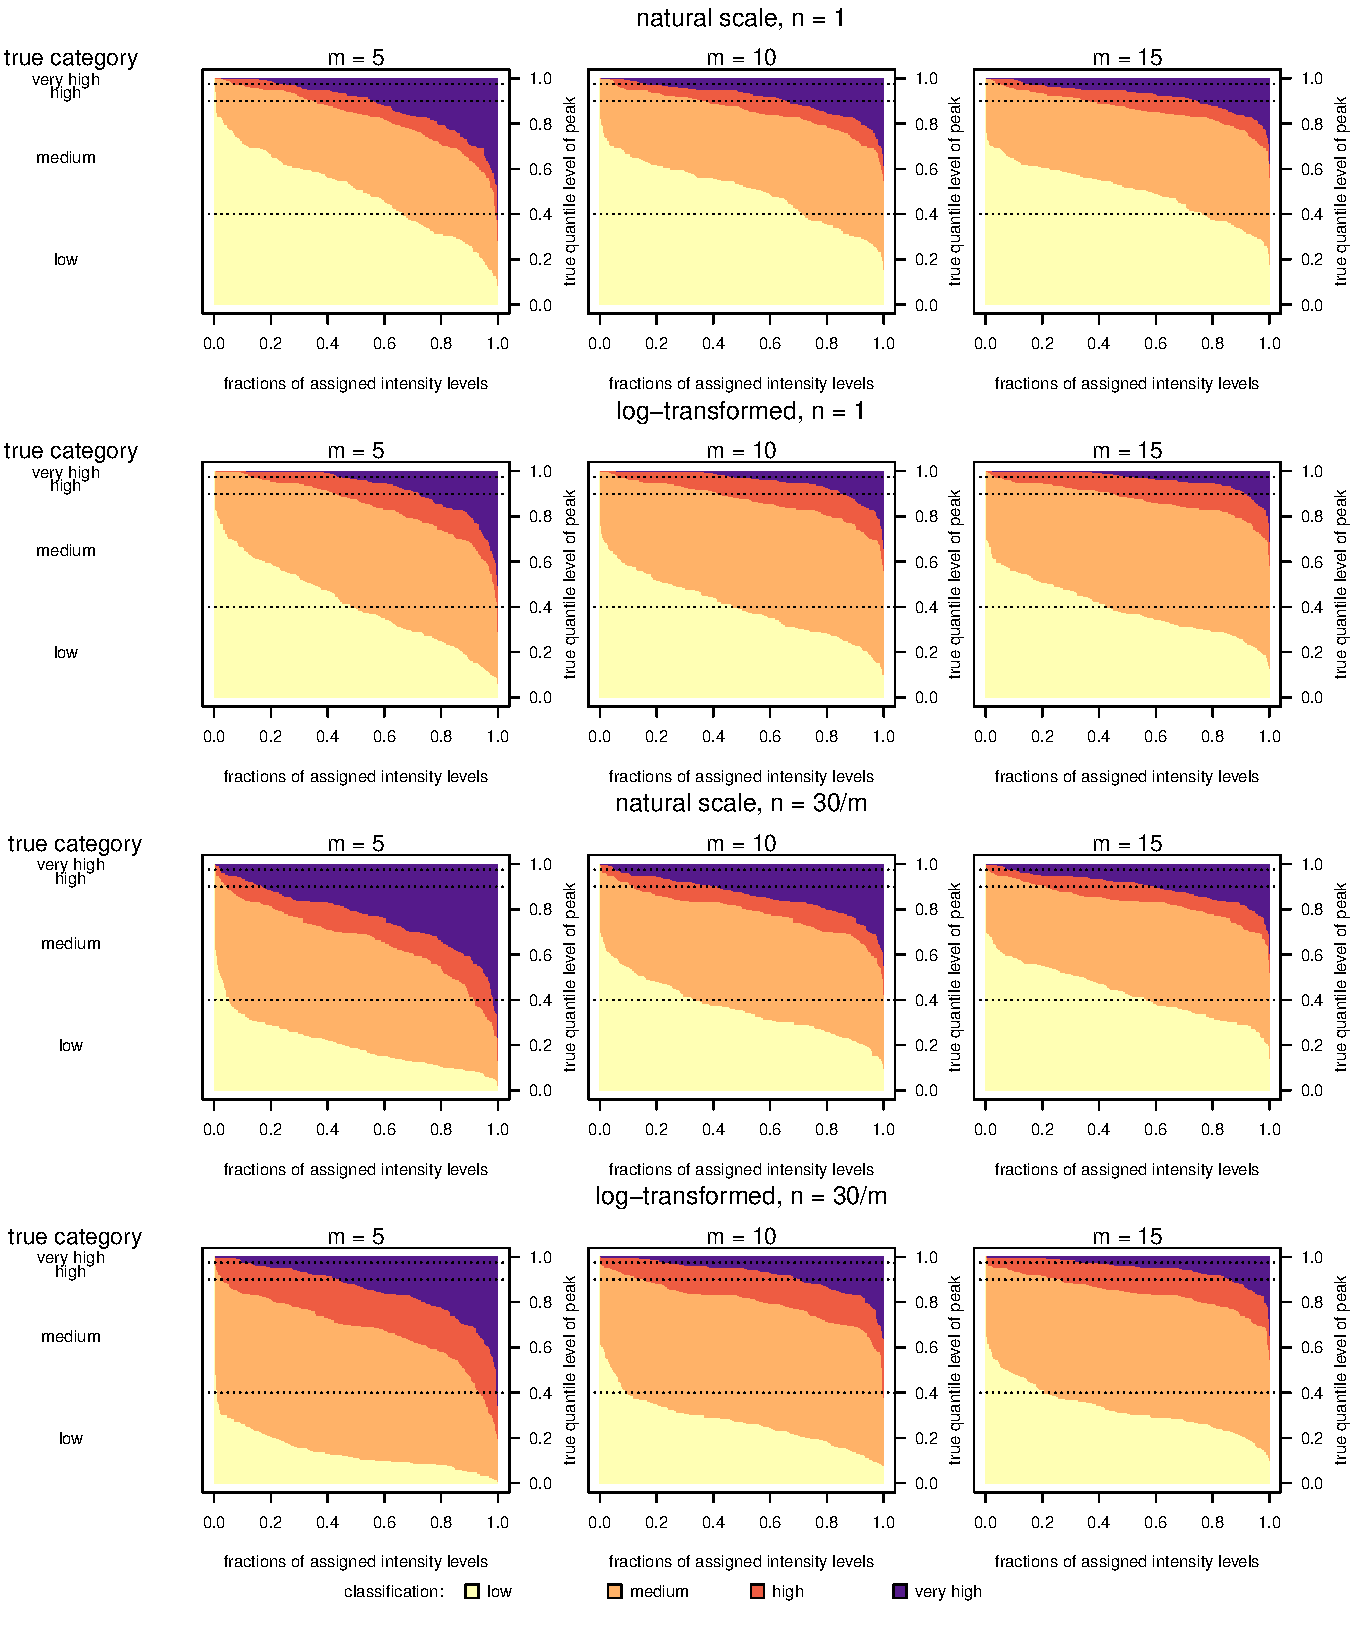
\includegraphics[width=0.9\textwidth]{figure/mosaic_fr_fancy.pdf}
\caption{Intensity classifications obtained with different choices of $n$ and transformation function $f$, as a function of the true quantile level of a season peak (i.e., with respect to the true distribution). This corresponds to a more detailed version of Figure \ref{fig:mosaic}.}
\label{fig:mosaic_fancy}
\end{figure}

\newpage

\begin{figure}[h!]
\center
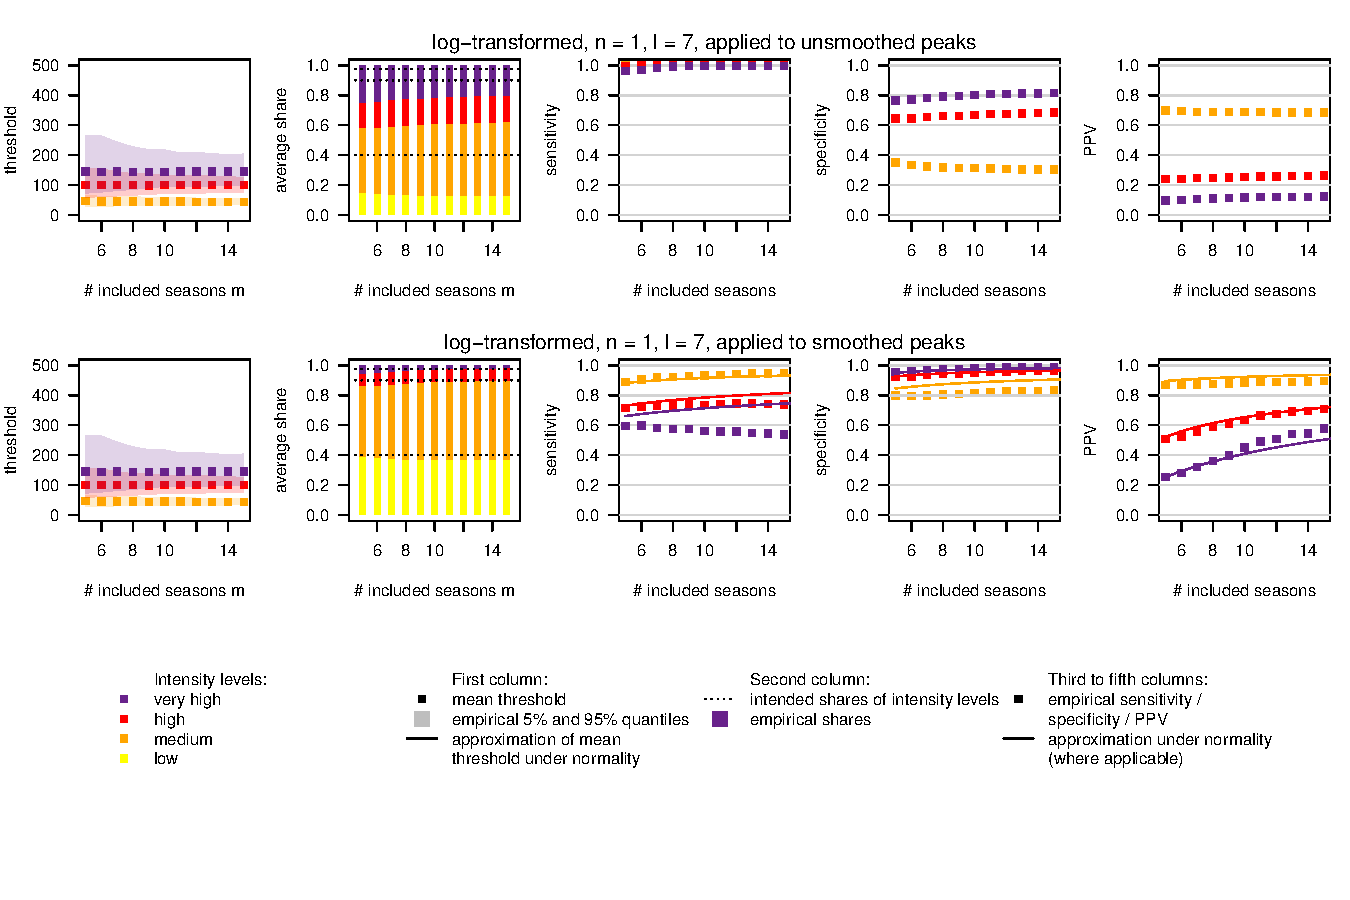
\includegraphics[width=0.85\textwidth]{figure/plot_smoothing7_fr_small.pdf}
\caption{Impact of smoothing of historical data on thresholds. We applied a moving average with $l = 7$ to the historical time series prior to computing thresholds and subsequently applied them to either unsmoothed or smoothed new peak values. Results are shown for thresholds computed with a log transformation. See the legend of Figure \ref{fig:results1} for details on the plot elements.}
\label{fig:results_smoothing7}
\end{figure}


\begin{figure}[h!]
\begin{center}
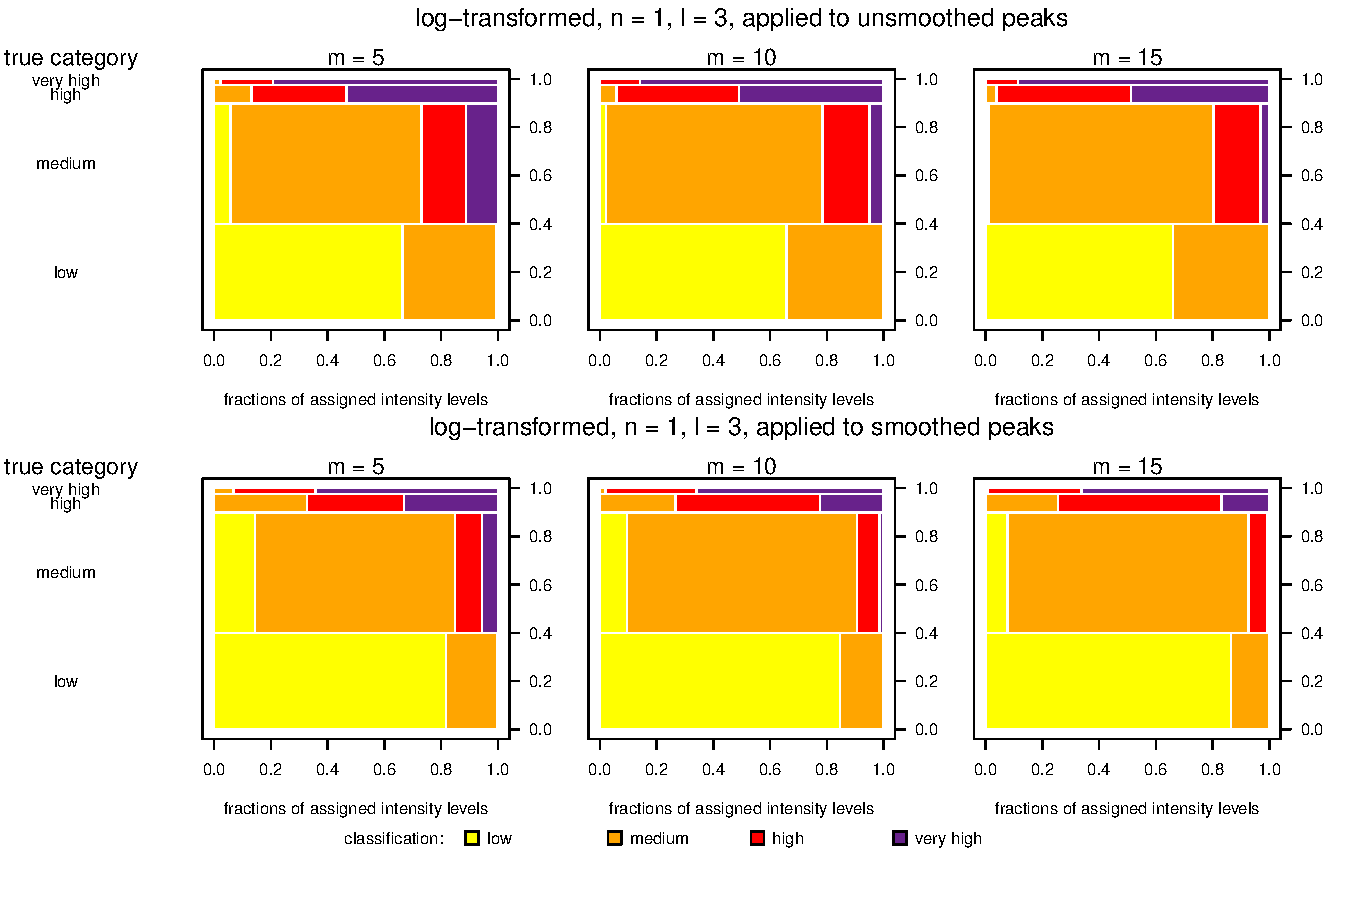
\includegraphics[width=0.7\textwidth]{figure/mosaic_log_smoothed_fr.pdf}

\caption{Confusion matrices for intensity classifications obtained with a smoothing window of width $l = 3$ and a log transformation. Top: thresholds applied to unsmoothed new peaks; bottom: thresholds applied to smoothed new peaks. Mosaic plots show which fractions of season peaks which are truly very high, high, medium or low are classified into the four categories, see caption of Figure \ref{fig:mosaic} for details.}
\label{fig:mosaic_smoothing}
\end{center}
\end{figure}

\newpage


\begin{figure}[h!]
\begin{center}
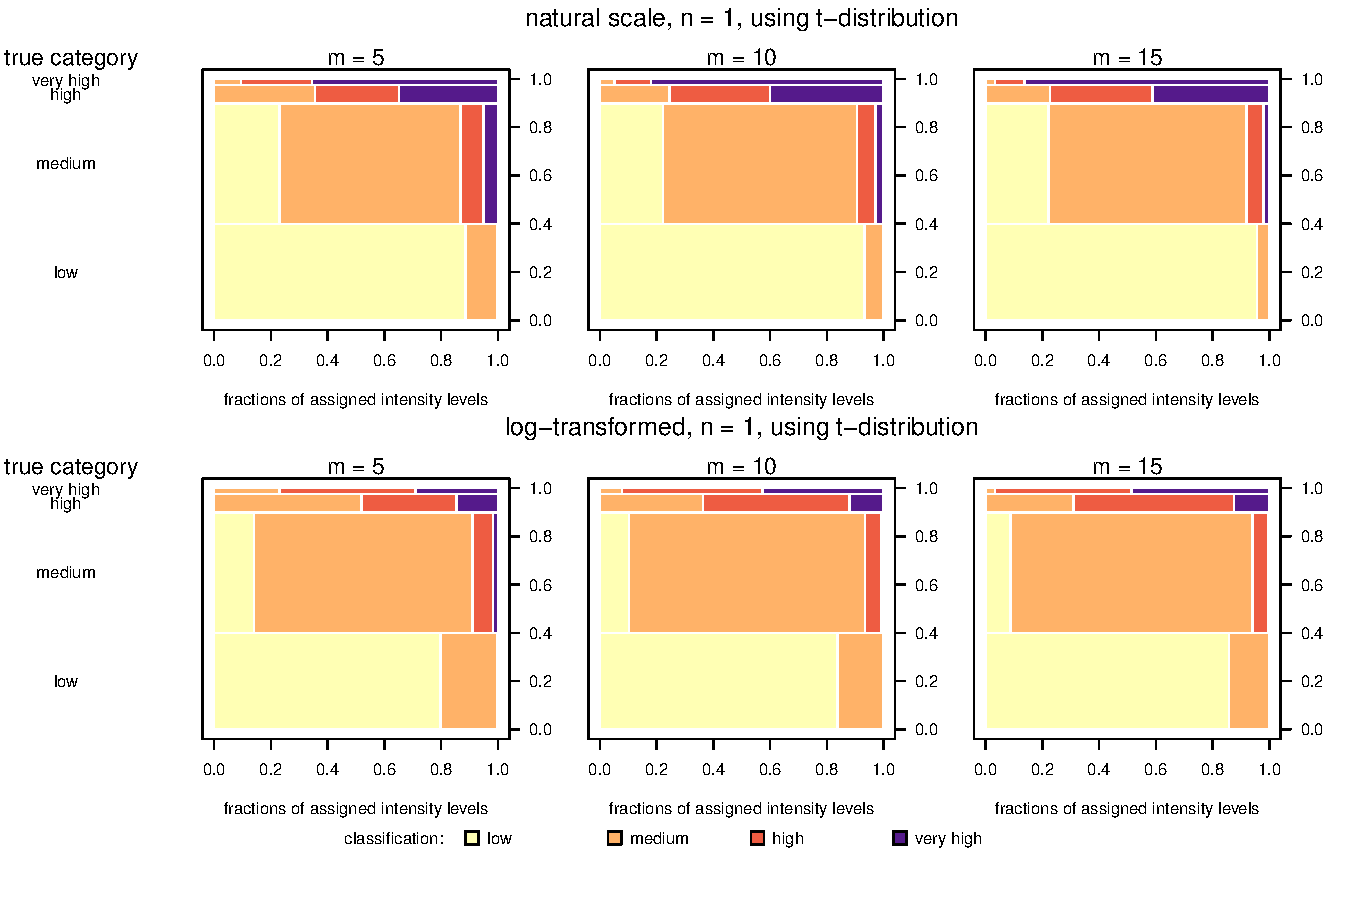
\includegraphics[width=0.7\textwidth]{figure/mosaic_t_fr.pdf}

\caption{Confusion matrices for intensity classifications based on quantiles of a $t$ rather than normal distribution. Mosaic plots show which fractions of season peaks which are truly very high, high, medium or low are classified into the four categories, see caption of Figure \ref{fig:mosaic} for details.}
\label{fig:mosaic_t}
\end{center}
\end{figure}

%\begin{figure}[h!]
%\begin{center}
%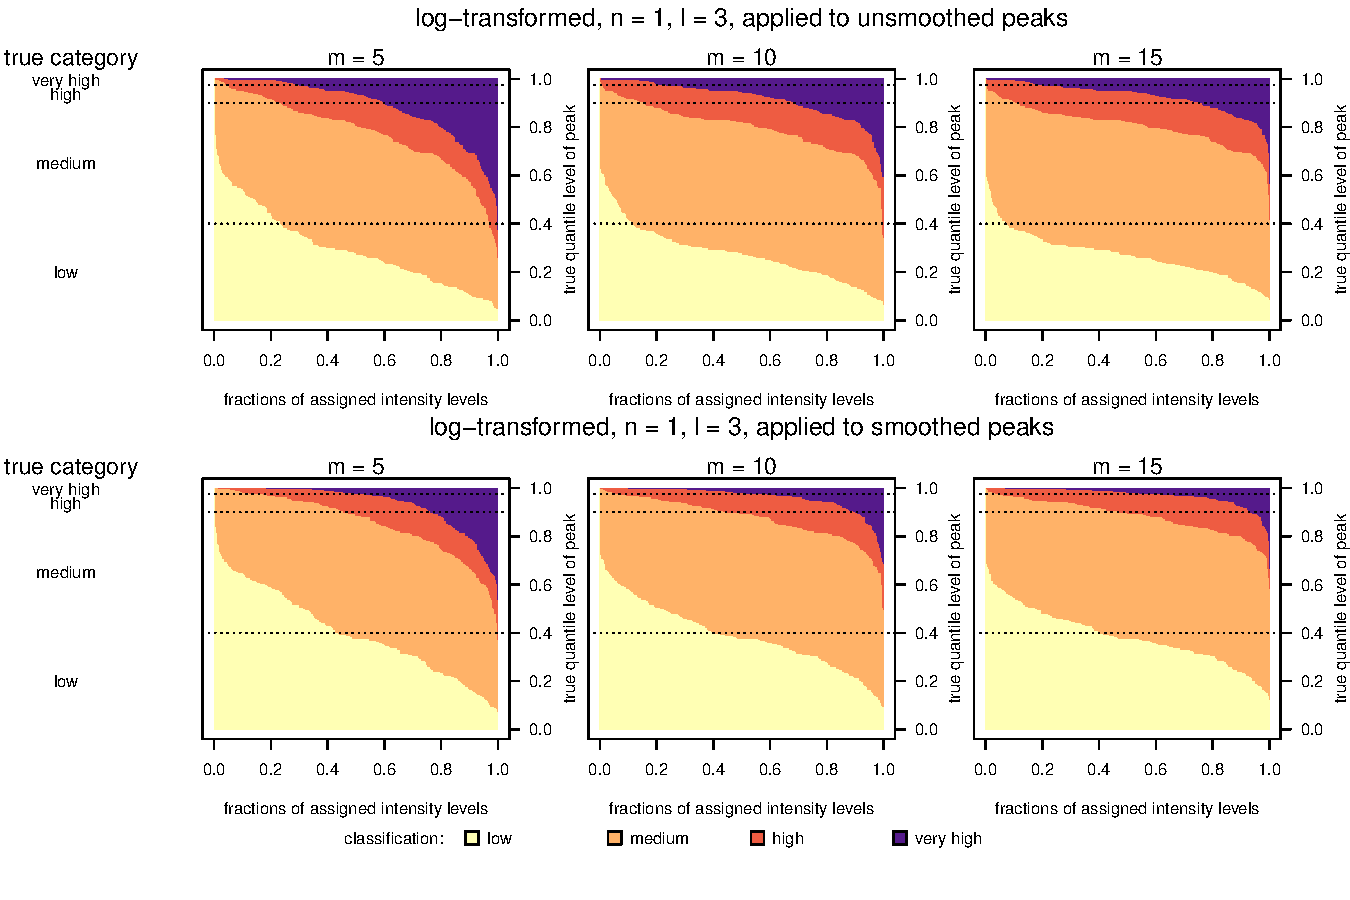
\includegraphics[width=0.7\textwidth]{figure/mosaic_log_smoothed_fr_fancy.pdf}
%\caption{Intensity classifications obtained with a smoothing window of width $l = 3$ and a log transformation, as a function of the true quantile level of a season peak (i.e., with respect to the true distribution). This corresponds to a more detailed version of Figure \ref{fig:mosaic_smoothing}. Top: thresholds applied to unsmoothed new peaks; bottom: thresholds applied to smoothed new peaks.}
%\label{fig:mosaic_smoothing_fancy}
%\end{center}
%\end{figure}


\begin{figure}[h!]
\begin{center}
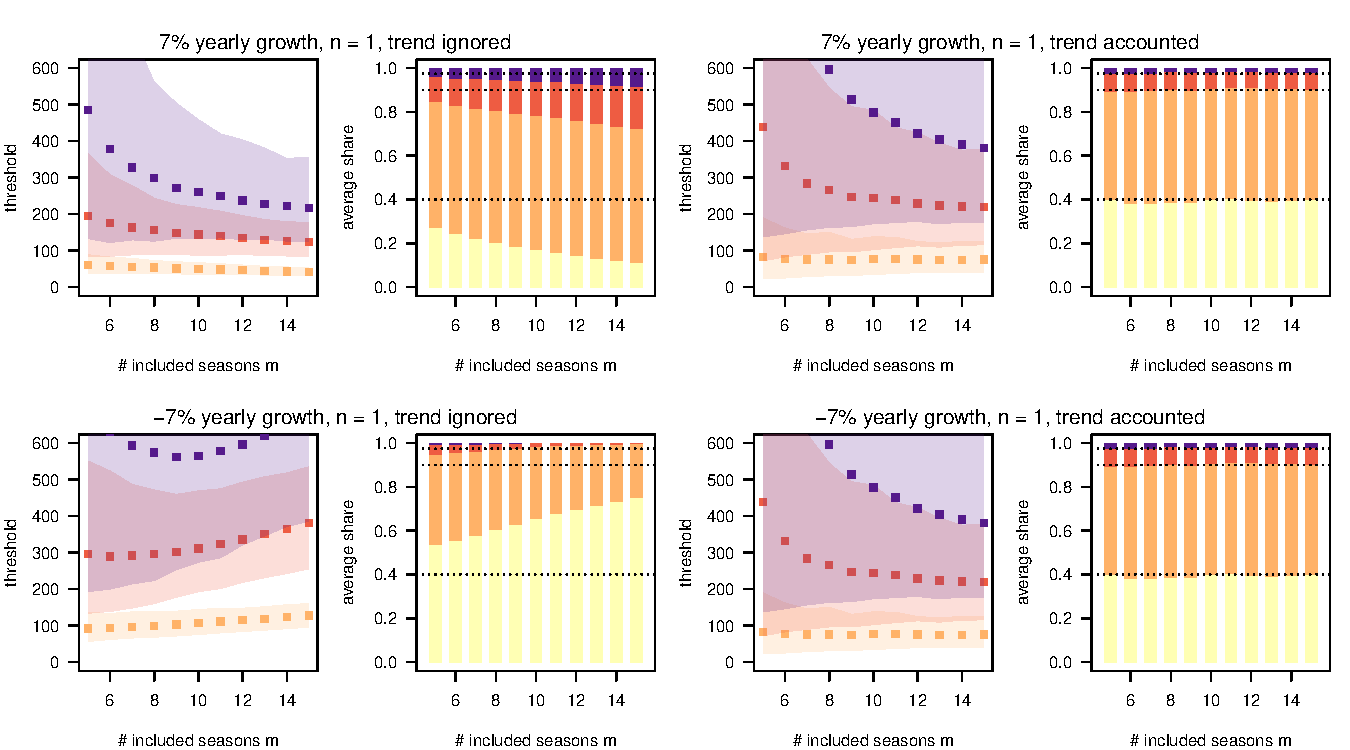
\includegraphics[width = 0.9\textwidth]{figure/plot_trend7_fr_small.pdf}
\end{center}
\caption{Average thresholds and exceedance shares in the presence of constant annual growth (7\%) and decrease (-7\%). In each setting we computed thresholds with and without accounting for the secular trend. This parallels Figure \ref{fig:trend}.}
\label{fig:trend7}
\end{figure}

\newpage


\begin{figure}[h!]
\begin{center}
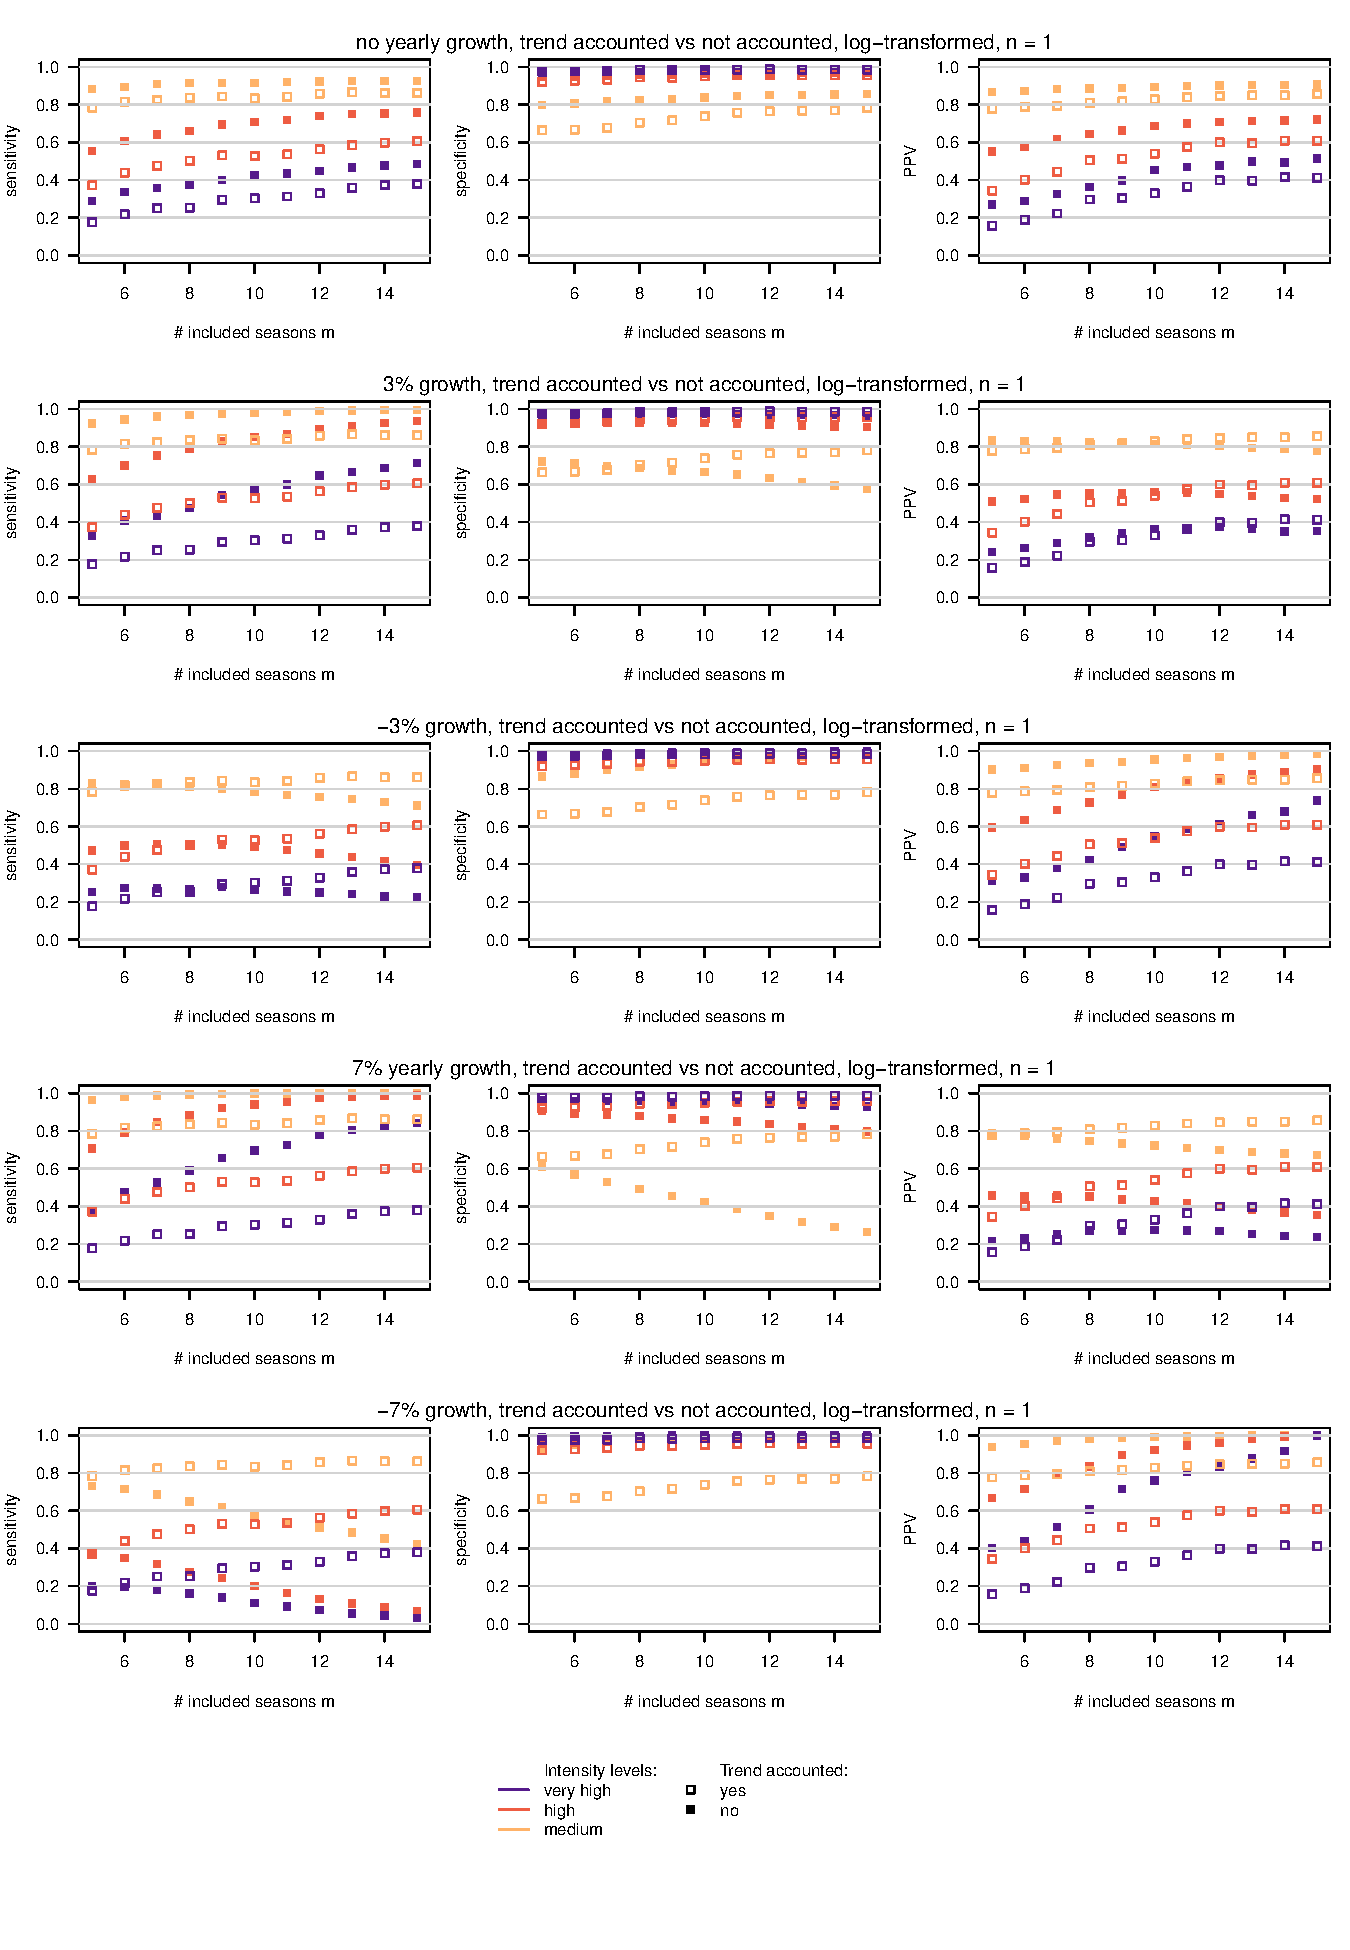
\includegraphics[width = 0.8\textwidth]{figure/plot_cost_trend_fr.pdf}
\end{center}
\vspace{-10mm}
\caption{Sensitivity, specificity and positive predictive values in three settings involving secular trends. Top row: no true secular trend. Second and third row: secular trend with a yearly growth rate of $\pm 3\%$. Fourth and fifth row: Secular trend with a yearly growth rate of $\pm 7\%$. In each plot we display the respective values as a function of $m$ and whether the secular trend was accounted for in thresholds or not (filled squares: not accounted; unfilled: accounted).}
\label{fig:cost_trend}
\end{figure}

\newpage

\section{Supplementary figures based on US data}
\label{suppl:us}

In the following, Figures \ref{fig:data}--\ref{fig:cis} are reproduced using the data from the US described in Section \ref{subsec:data}.

\begin{figure}[h]
\center
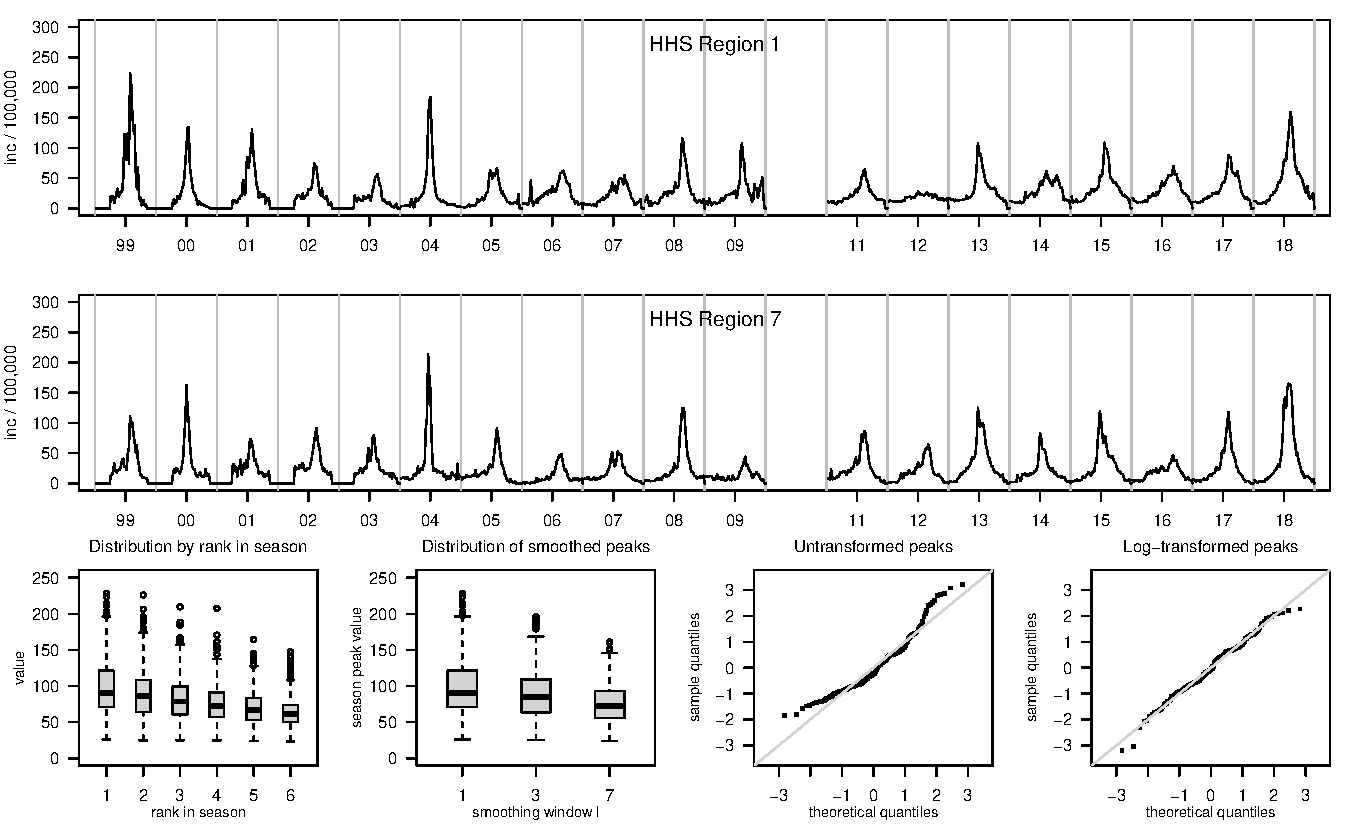
\includegraphics[width=1\textwidth]{figure/plot_data_us.pdf}
\caption{Reproduction of Figure \ref{fig:data} using US data. Re-scaled Time series of weekly weighted ILI percentages in US HHS Regions 1 and 7, 1999--2018. Off-season weeks are omitted in the plot, with grey lines delimiting the different seasons. The bottom row shows descriptive plots of the distribution of season peaks. First: Boxplots of values by rank within season. Second: Boxplot of smoothed peak values as a function of the smoothing window width $l$. Third: Normal QQ plot of untransformed peak values. Fourth: Normal QQ plot of log-transformed peak values.}
\label{fig:data_us}
\end{figure}

\newpage

\begin{figure}[h!]
\centering
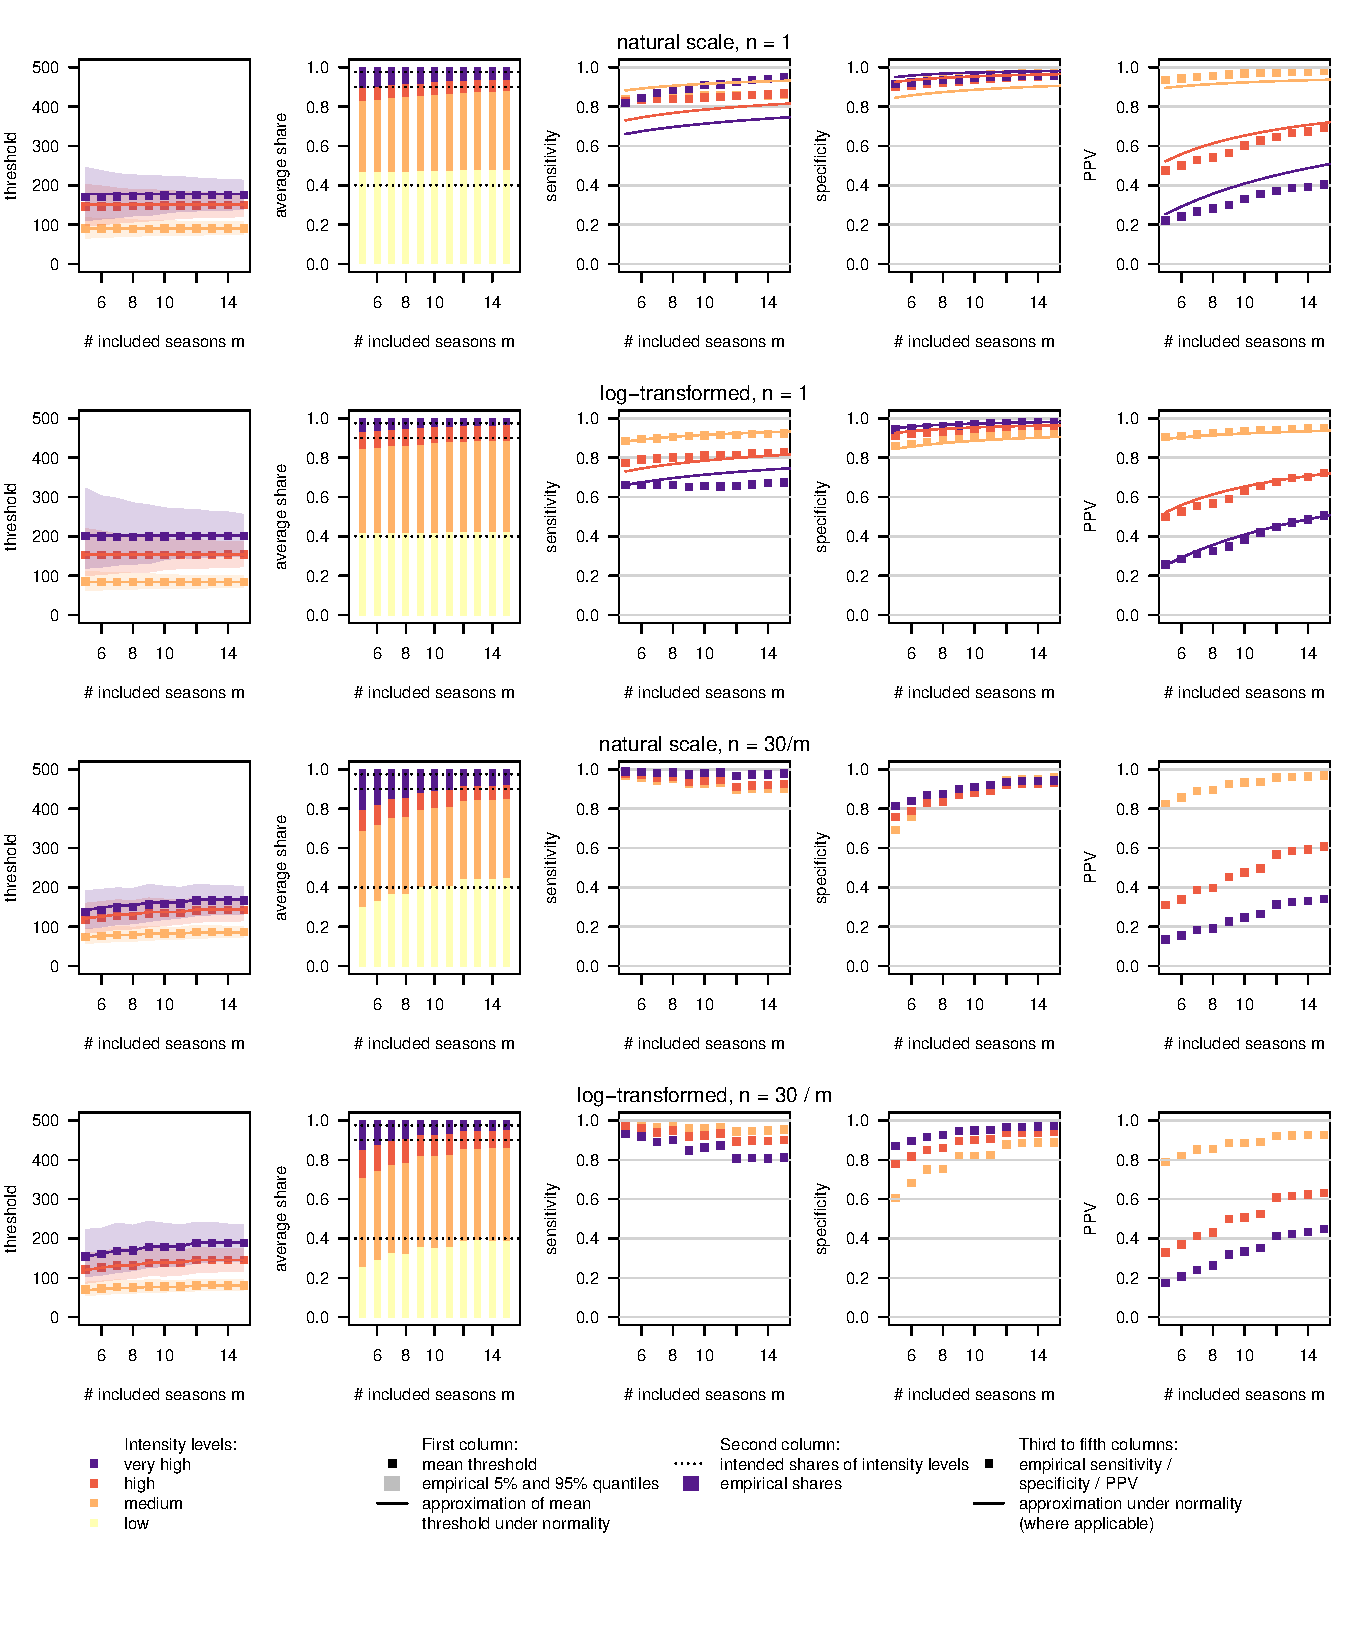
\includegraphics[width=0.9\textwidth]{figure/plot_us.pdf}

\vspace{-1.5cm}

\caption{Reproduction of Figure \ref{fig:results1} using US data. Impact of the choice of $n$ and transformation function $f$. First column: simulation-based average intensity thresholds (squares) along with bands delimited by the empirical 5\% and 95\% quantiles. Analytical approximations of mean threshold values (computed from empirical means and covariance matrices) are displayed as lines. Second column: resulting average shares of season peaks classified as low, medium, high and very high intensity. Third to fifth columns: sensitivity, specificity and PPVs of the different thresholds. Simulation results are shown as squares. Where available analytical approximations are shown as lines.}
\label{fig:results1_us}
\end{figure}

\newpage

\begin{figure}[h!]
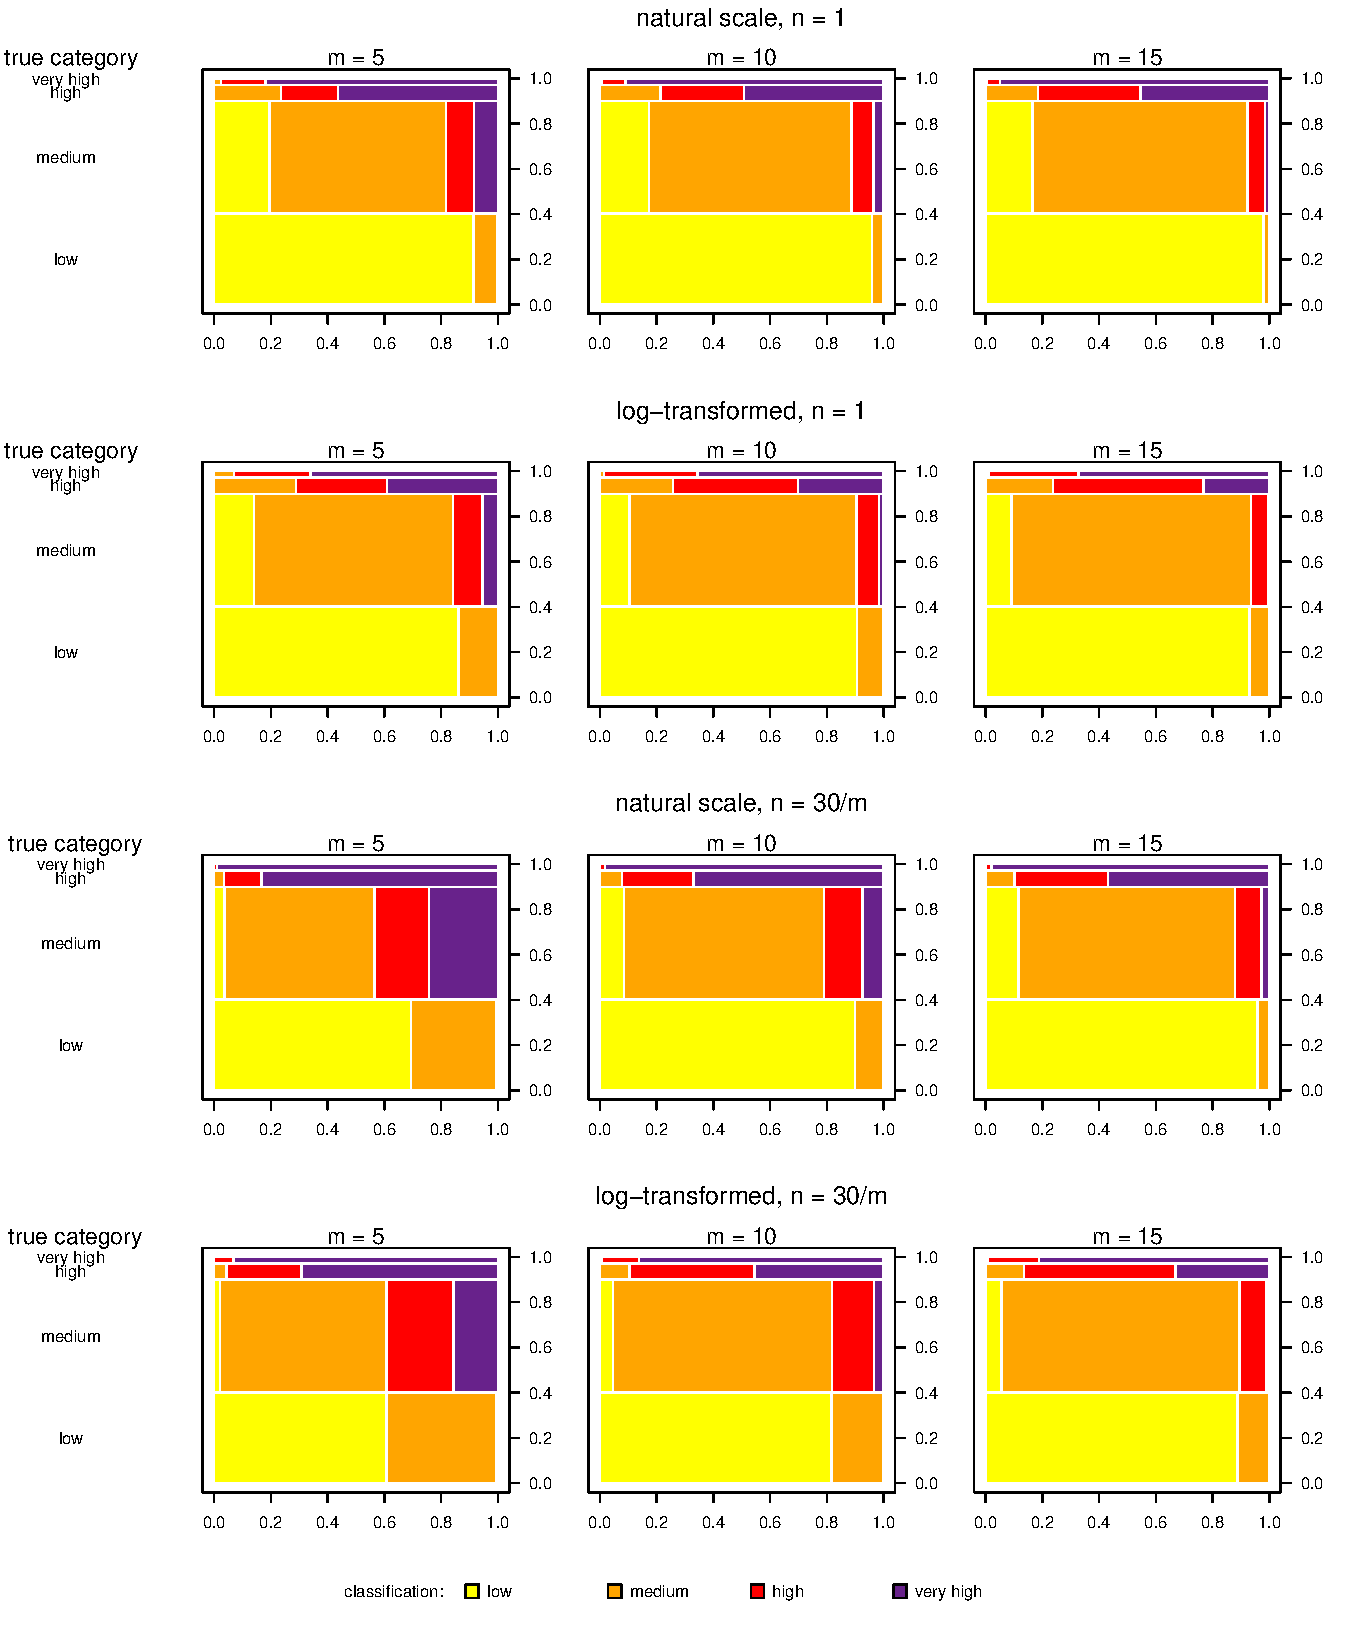
\includegraphics[width=0.9\textwidth]{figure/mosaic_us.pdf}
\caption{Reproduction of Figure \ref{fig:mosaic} using US data. Confusion matrices for intensity classifications obtained with different choices of $n$ and transformation function $f$. Mosaic plots show which fractions of season peaks which are truly very high, high, medium or low are classified into the four categories. The true class is determined with respect to the empirical quantiles of the distribution of peaks: very high (highest 2.5\% of all peaks), high (next 7.5\%), medium (next 50\%), low (lowest 40\% of all peaks).}
\label{fig:mosaic_us}
\end{figure}

\newpage 


\begin{figure}[h!]
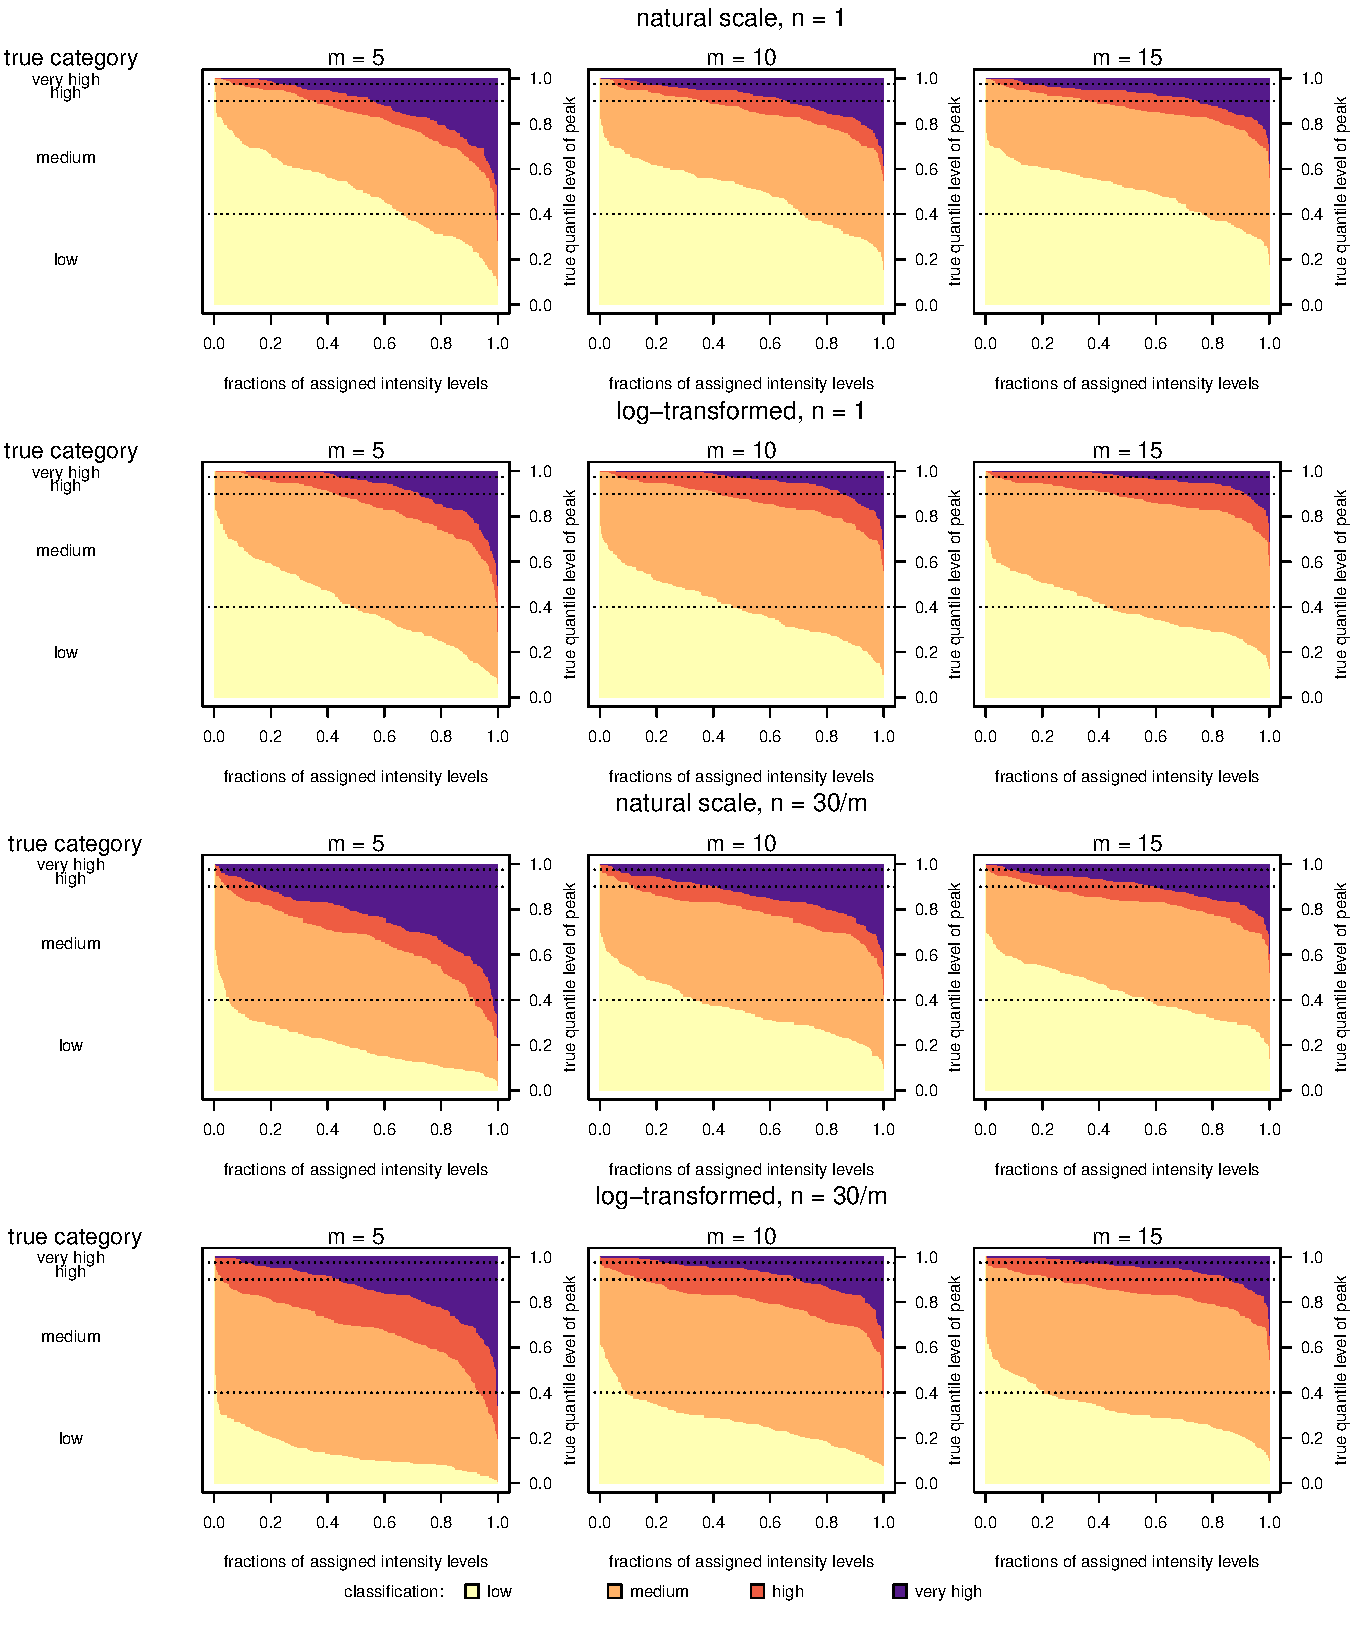
\includegraphics[width=0.9\textwidth]{figure/mosaic_fr_fancy.pdf}
\caption{Reproduction of Figure \ref{fig:mosaic_fancy} using US data. Intensity classifications obtained with different choices of $n$ and transformation function $f$, as a function of the true quantile level of a season peak (i.e., with respect to the true distribution). This corresponds to a more detailed version of Figure \ref{fig:mosaic_us}.}
\label{fig:mosaic_fancy_us}
\end{figure}

\newpage

\begin{figure}[h!]
\centering
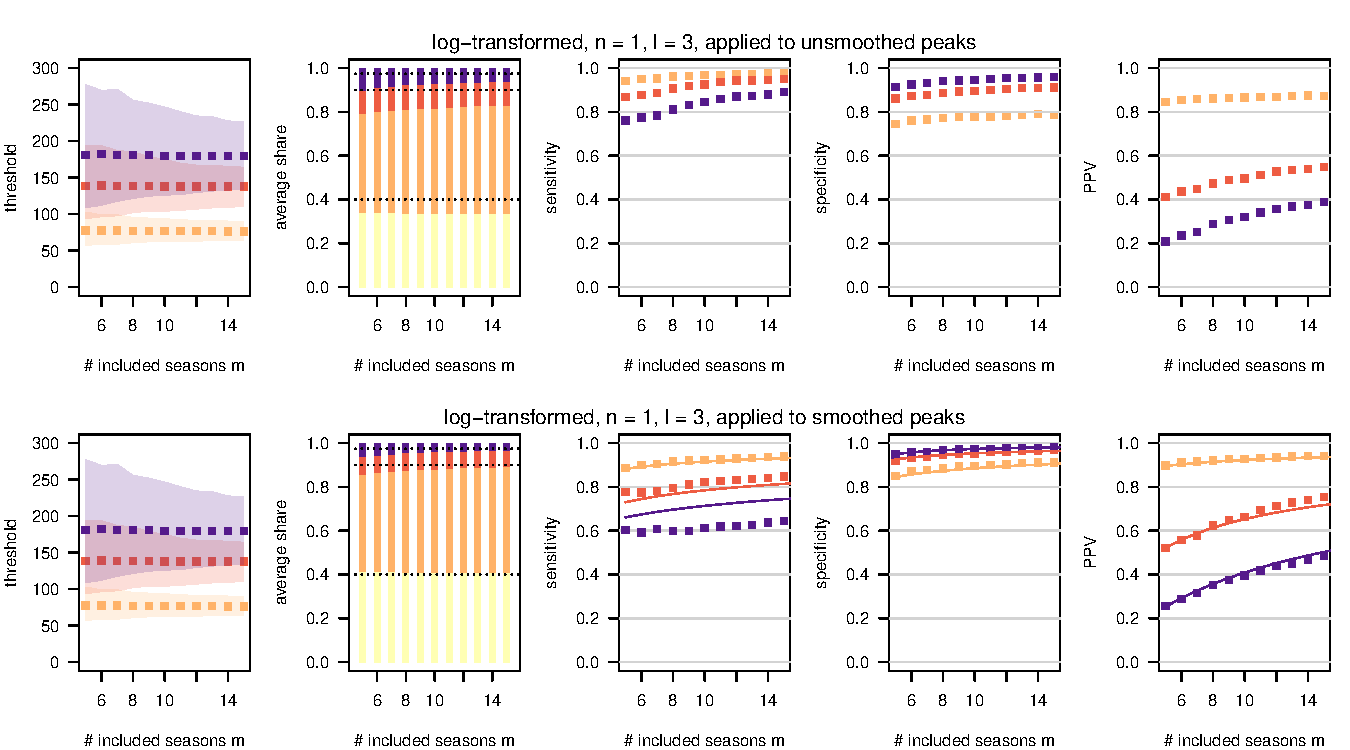
\includegraphics[width=0.85\textwidth]{figure/plot_smoothing3_us_small.pdf}

\caption{Reproduction of Figure \ref{fig:results_smoothing} using US data. Impact of smoothing of historical data on thresholds. We applied a moving average with $l = 3$ to the historical time series prior to computing thresholds and subsequently applied them to either unsmoothed or smoothed new peak values. Results are shown for thresholds computed with a log transformation. See the caption of Figure \ref{fig:results1} for details on the plot elements.}
\label{fig:results_smoothing_us}
\end{figure}



\begin{figure}[h!]
\begin{center}
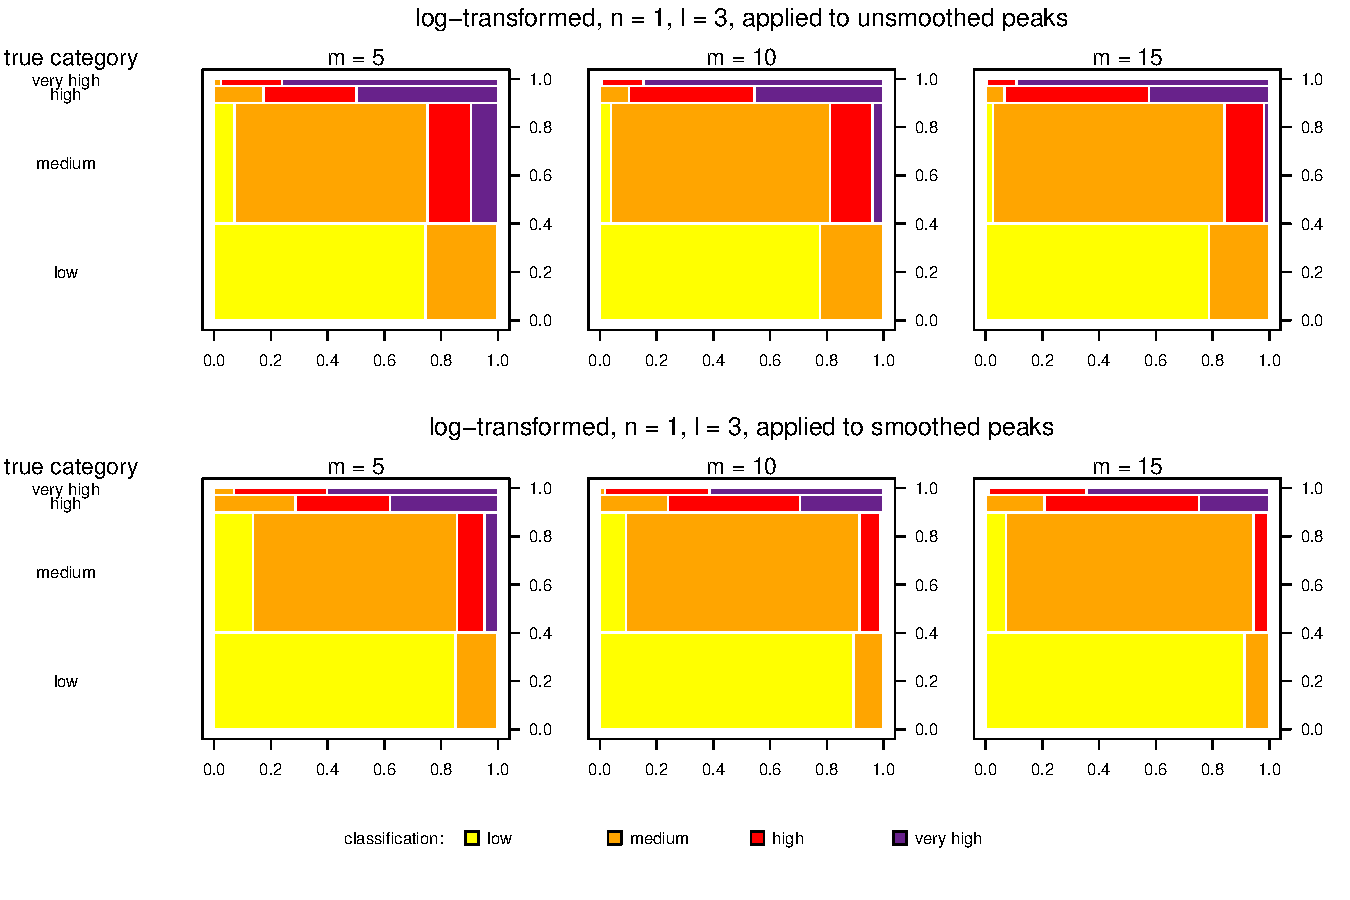
\includegraphics[width=0.7\textwidth]{figure/mosaic_log_smoothed_us.pdf}
\end{center}
\caption{Reproduction of Figure \ref{fig:mosaic_smoothing} using US data. Confusion matrices for intensity classifications obtained with a smoothing window of width $l = 3$ and a log transformation. Top: thresholds applied to unsmoothed new peaks; bottom: thresholds applied to smoothed new peaks. Mosaic plots show which fractions of season peaks which are truly very high, high, medium or low are classified into the four categories, see caption of Figure \ref{fig:mosaic} for details.}
\label{fig:mosaic_smoothing_us}
\end{figure}


\newpage


\begin{figure}[h!]
\begin{center}
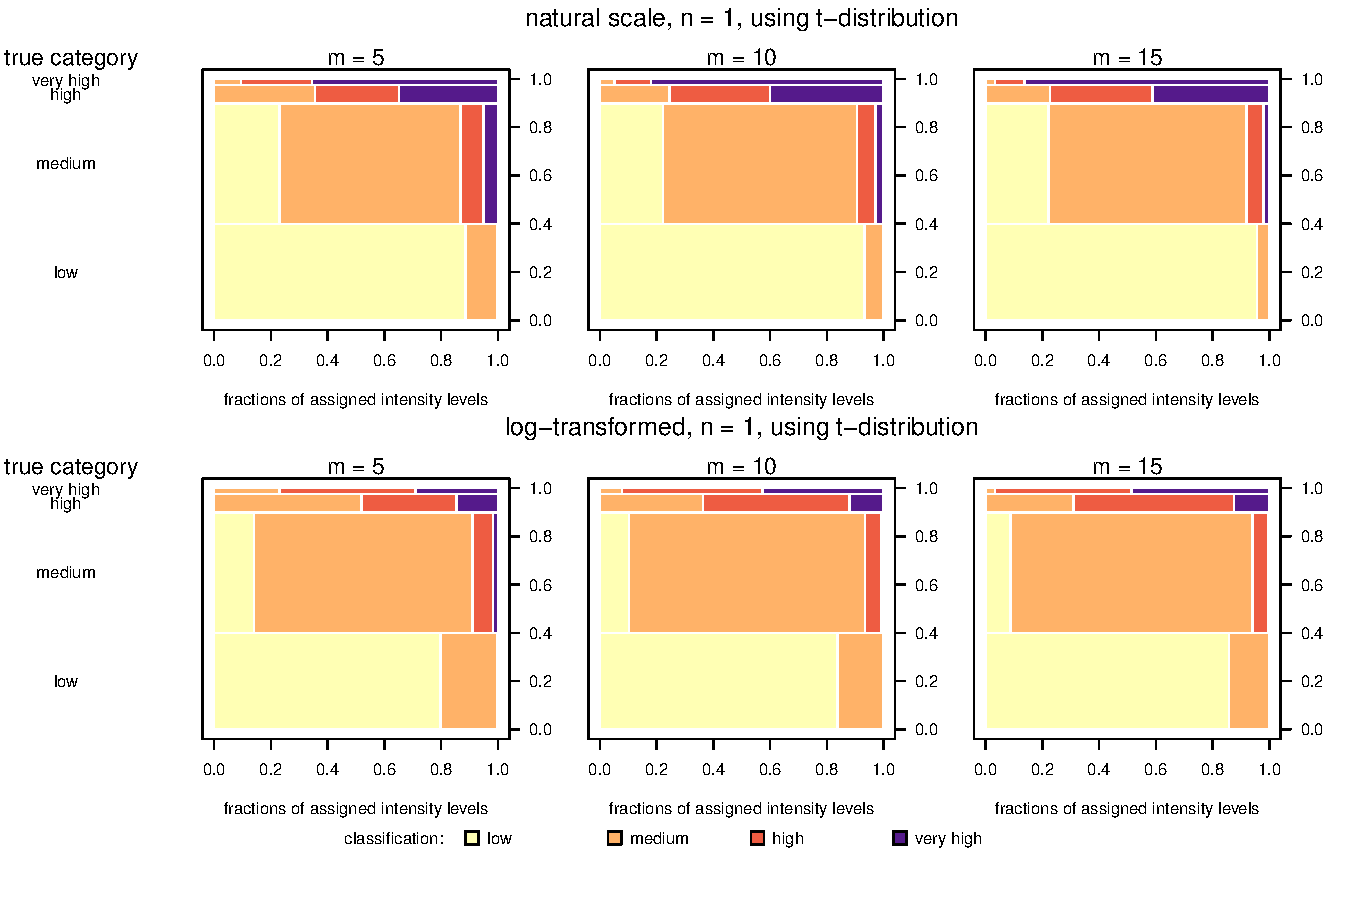
\includegraphics[width=0.7\textwidth]{figure/mosaic_t_fr.pdf}

\caption{Reproduction of Figure \ref{fig:mosaic_t} using US data. Confusion matrices for intensity classifications based on quantiles of a $t$ rather than normal distribution. Mosaic plots show which fractions of season peaks which are truly very high, high, medium or low are classified into the four categories, see caption of Figure \ref{fig:mosaic} for details.}
\label{fig:mosaic_t_us}
\end{center}
\end{figure}



\begin{figure}[h!]
\begin{center}
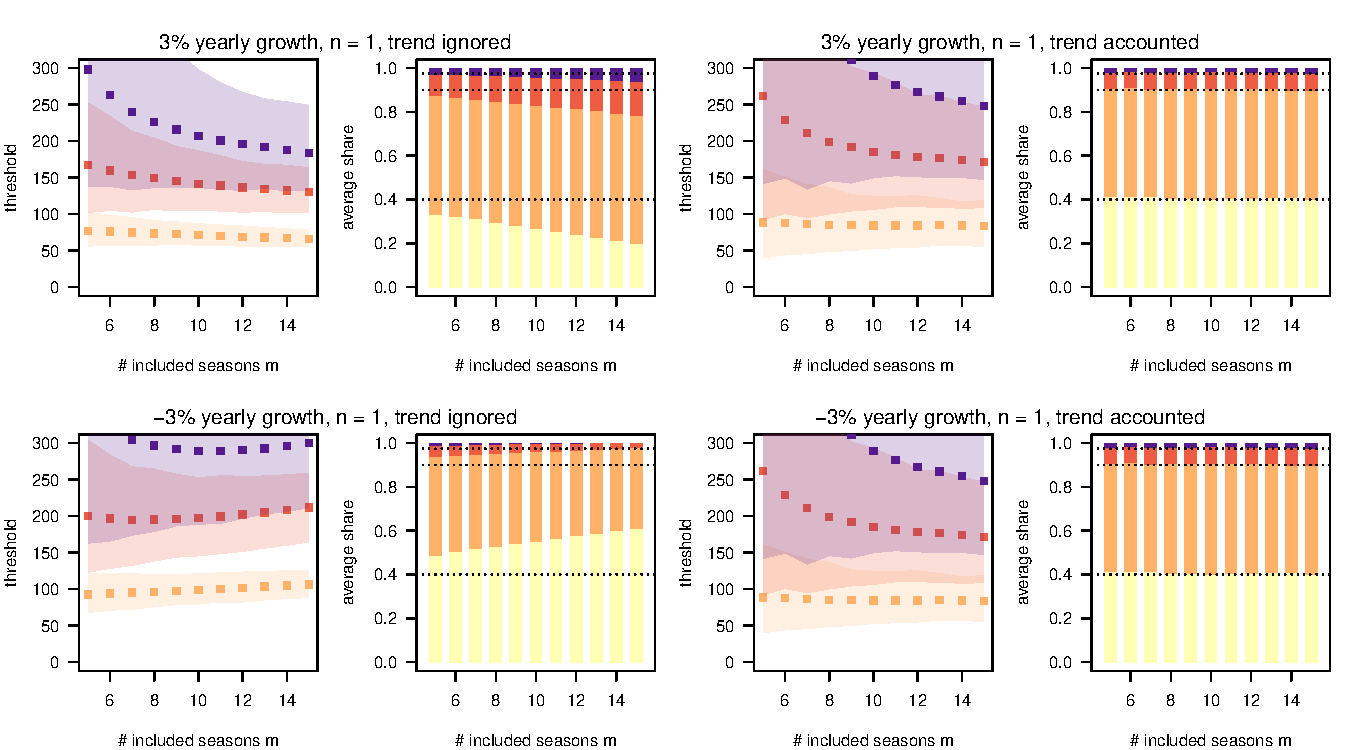
\includegraphics[width = 0.9\textwidth]{figure/plot_trend3_us_small.pdf}
\end{center}
\caption{Reproduction of Figure \ref{fig:trend} using US data. Average thresholds and exceedance shares in the presence of constant annual growth (3\%) and decrease (-3\%). In each setting we computed thresholds with and without accounting for the secular trend.}
\label{fig:trend_us}
\end{figure}

\begin{figure}[h!]¨
\begin{center}
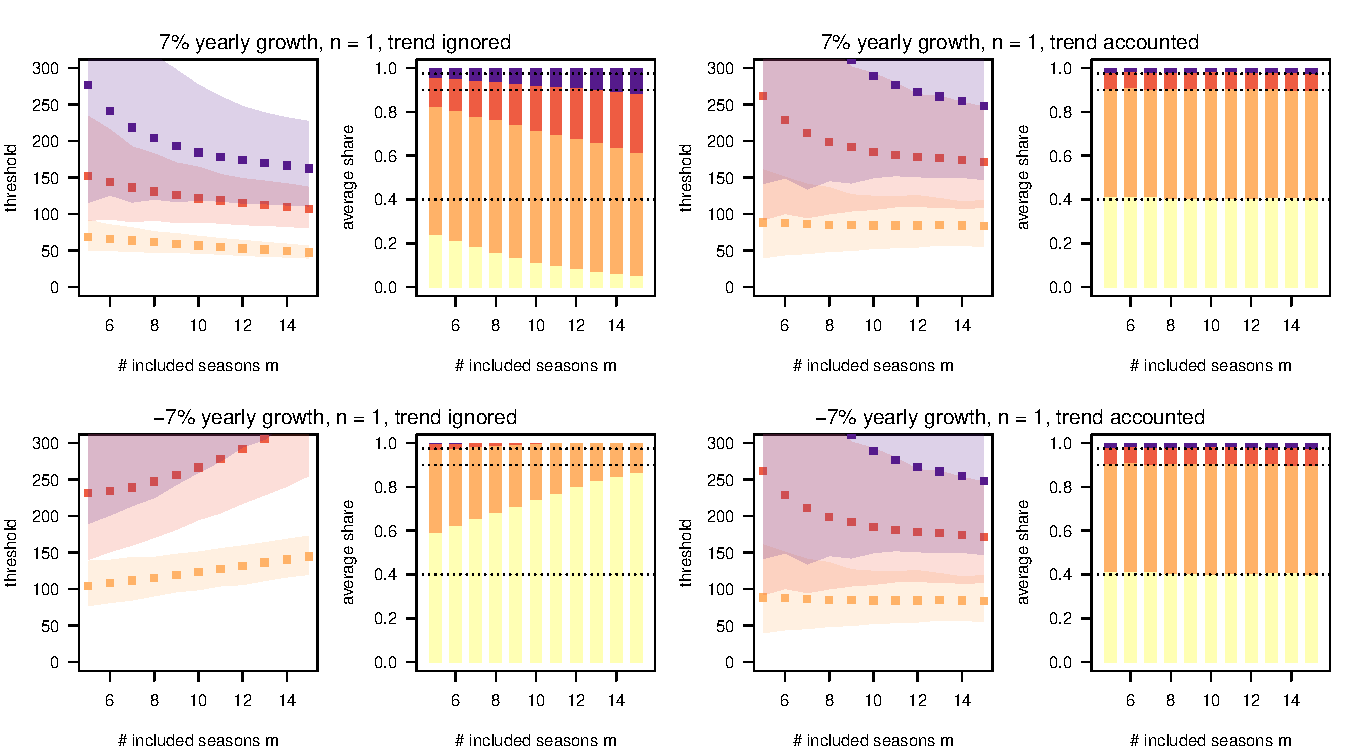
\includegraphics[width = 0.9\textwidth]{figure/plot_trend7_us_small.pdf}
\end{center}
\caption{Reproduction of Figure \ref{fig:trend7} using US data. Average thresholds and exceedance shares in the presence of constant annual growth (7\%) and decrease (-7\%). In each setting we computed thresholds with and without accounting for the secular trend. This parallels Figure \ref{fig:trend}.}
\label{fig:trend7_us}
\end{figure}


\newpage

\begin{figure}[h!]
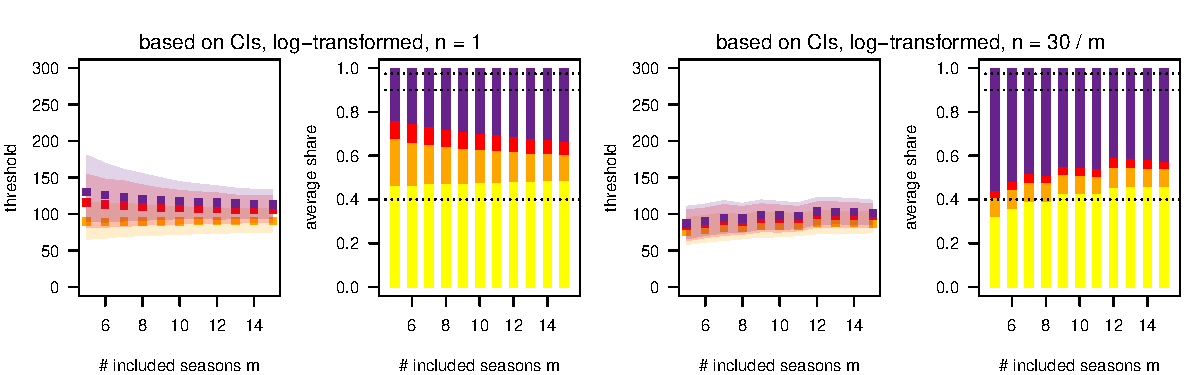
\includegraphics[width=0.93\textwidth]{figure/plot_ci_us.pdf}
\caption{Reproduction of Figure \ref{fig:cis} using US data. Average thresholds and exceedance shares when thresholds are based on confidence intervals rather than prediction intervals. See the caption and legend of Figure \ref{fig:results1} for details on the plot elements.}
\label{fig:cis_us}
\end{figure}

\newpage



\begin{figure}[h!]
\begin{center}
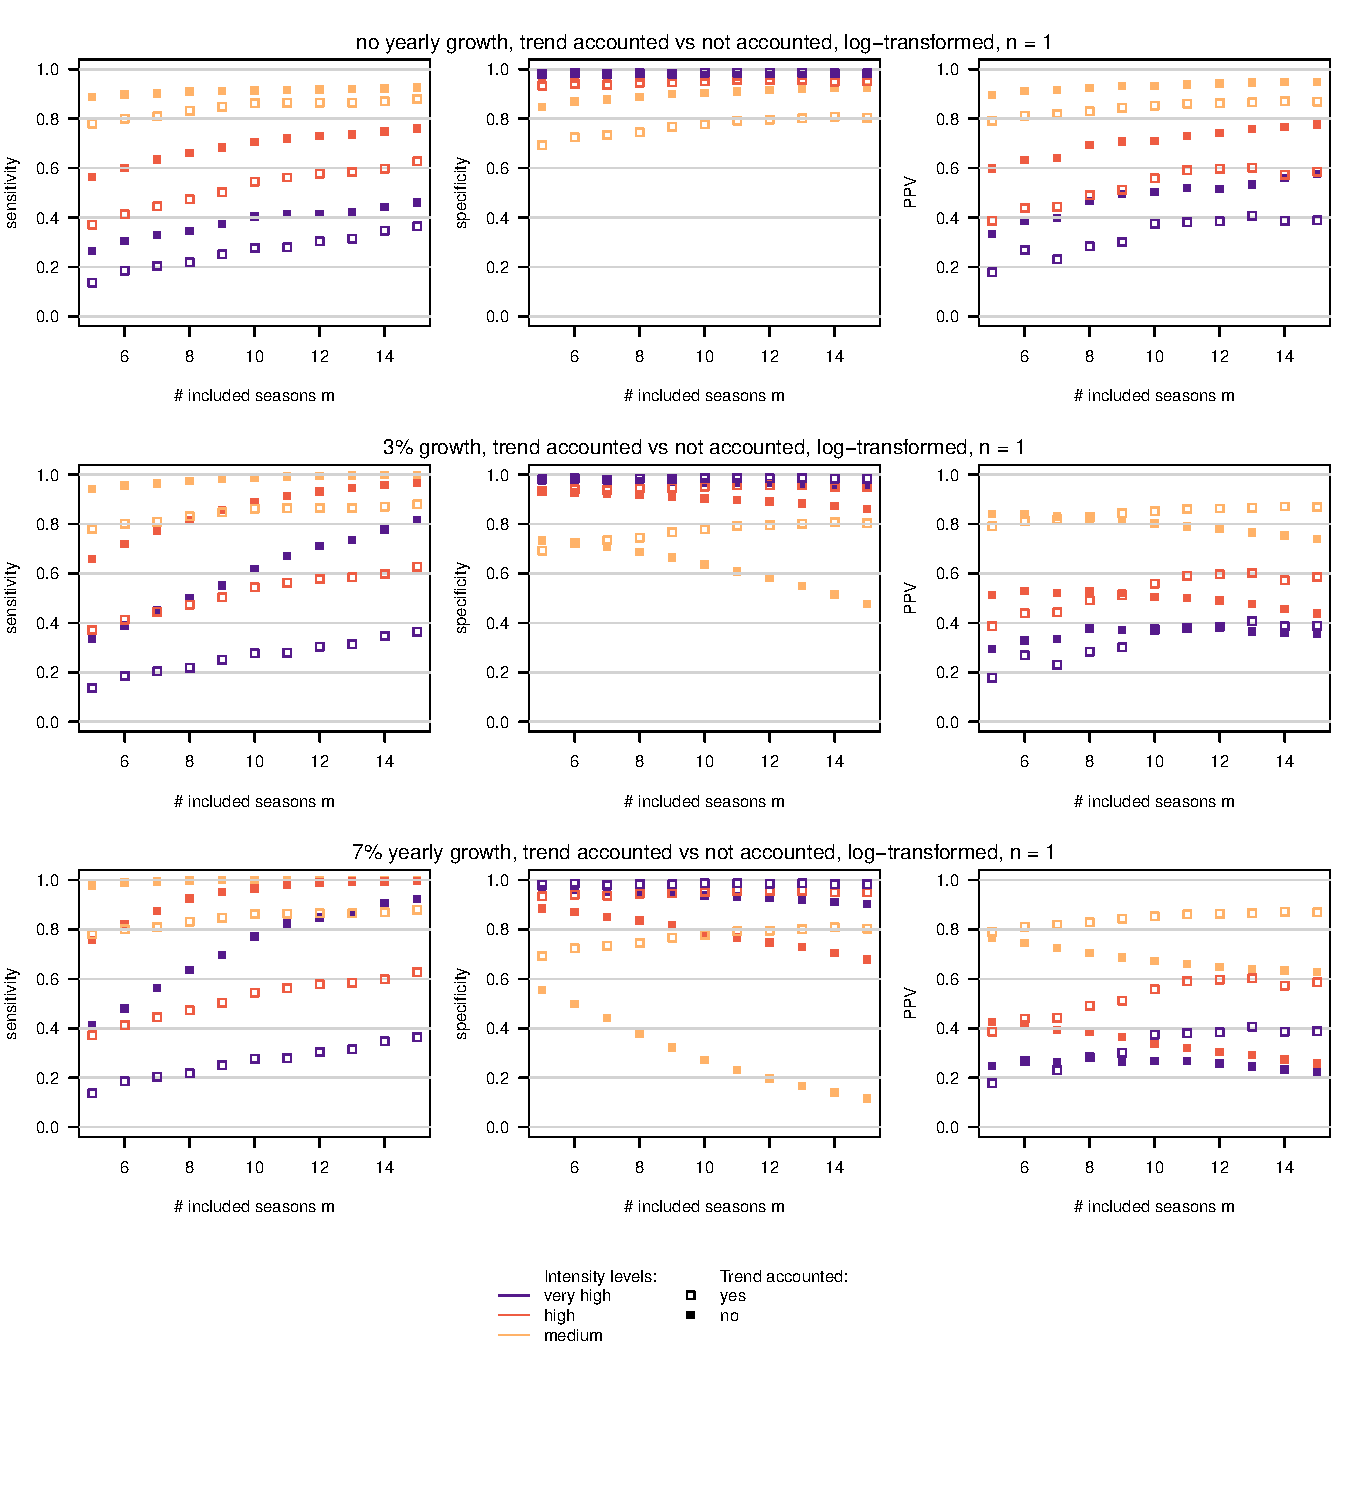
\includegraphics[width = 0.95\textwidth]{figure/plot_cost_trend_us.pdf}
\end{center}
\caption{Reproduction of Figure \ref{fig:cost_trend} using US data. Sensitivity, specificity and positive predictive values in three settings involving secular trends. Top row: now true secular trend. Middle row: secular trend with a yearly growth rate of 3\%. Bottom: Secular trend with a yearly growth rate of 7\%. In each plot we display the respective values as a function of $m$ and whether the secular trend was accounted for in thresholds or not (filled squares: not accounted; unfilled: accounted).}
\end{figure}

%\begin{figure}[h!]
%\begin{center}
%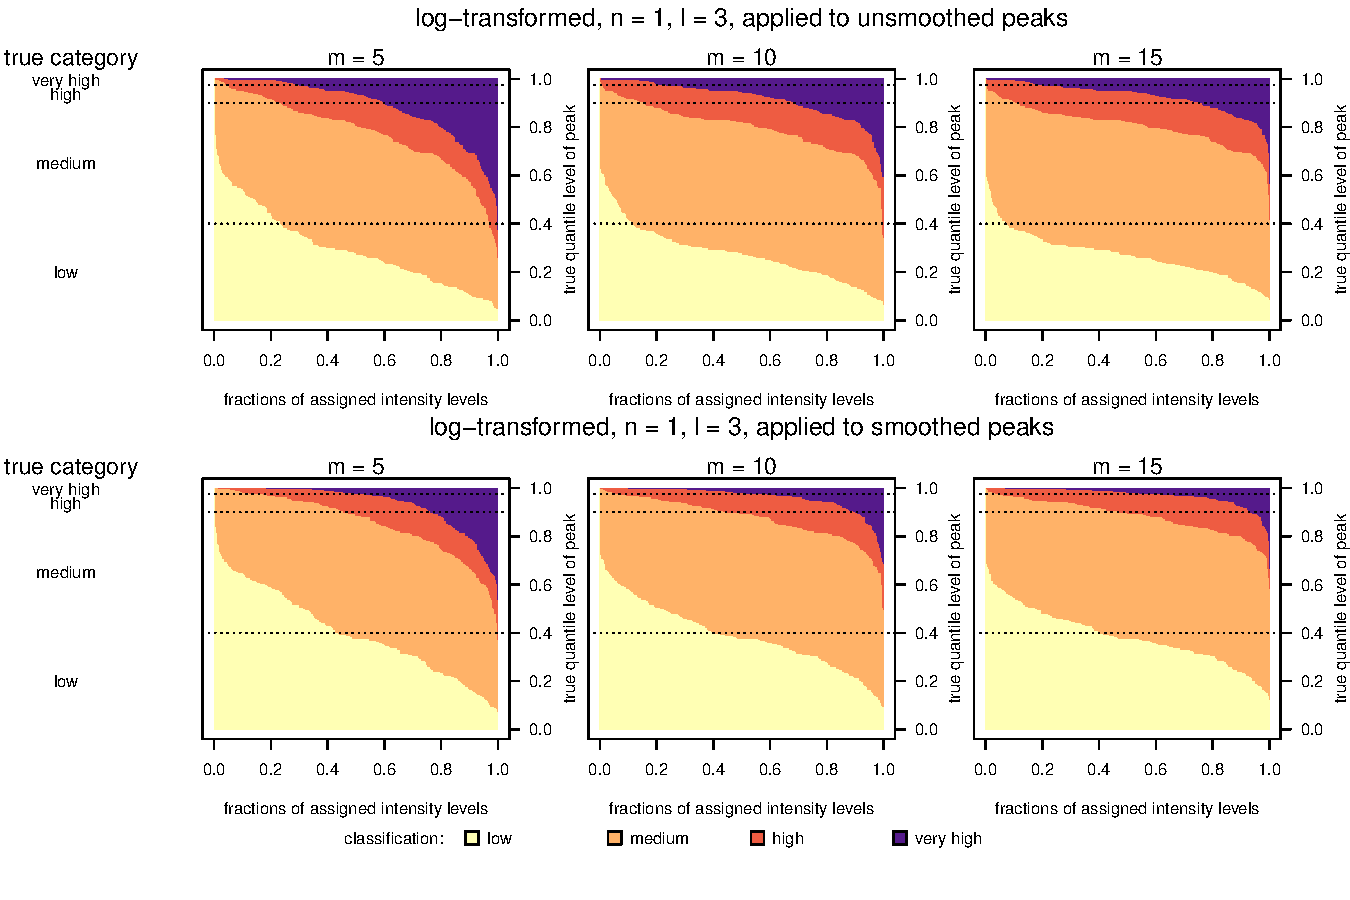
\includegraphics[width=0.87\textwidth]{figure/mosaic_log_smoothed_fr_fancy.pdf}
%\caption{Reproduction of Figure \ref{fig:mosaic_smoothing_us} using US data. Intensity classifications obtained with a smoothing window of width $l = 3$ and a log transformation, as a function of the true quantile level of a season peak (i.e., with respect to the true distribution). This corresponds to a more detailed version of Figure \ref{fig:mosaic_smoothing_us}. Top: thresholds applied to unsmoothed new peaks; bottom: thresholds applied to smoothed new peaks.}
%\label{fig:mosaic_smoothing_fancy_us}
%\end{center}
%\end{figure}






{\footnotesize
\bibliographystyle{apalike}
\bibliography{bibliography_mem}
}


\end{document}